\input{setup.tex}
% Режим шаблона (должен быть включен один из трех)
\ВКРtrue
%\Практикаtrue
%\Курсоваяtrue

\newcommand{\Дисциплина}{<<Проектирование и архитектура программных систем>>} % для курсовой
\newcommand{\КодСпециальности}{09.03.04} % Курсовая
\newcommand{\Специальность}{Программная инженерия} % Курсовая
\newcommand{\Тема}{Программная система с визуальной средой проектирования} % ВКР Курсовая
\newcommand{\ТемаВтораяСтрока}{для создания компьютерных игр}
\newcommand{\ГдеПроводитсяПрактика}{ООО «МЦОБ. Онлайн сервисе»} % для практики
\newcommand{\РуководительПрактПредпр}{} % для практики
\newcommand{\ДолжнРуководительПрактПредпр}{} % для практики
\newcommand{\РуководительПрактУнивер}{Чаплыгин А. А.} % для практики
\newcommand{\ДолжнРуководительПрактУнивер}{к.т.н. доцент} % для практики
\newcommand{\Автор}{Т. А. Дмитренко}
\newcommand{\АвторРод}{Дмитренко Т. А.}
\newcommand{\АвторПолностьюРод}{Дмитренко Тимура Александровича} % для практики
\newcommand{\Шифр}{22-06-0311}
\newcommand{\Курс}{4 } % для практики
\newcommand{\Группа}{ПО-22б}
\newcommand{\Руководитель}{А. В. Малышев} % для ВКР и курсовой
\newcommand{\Нормоконтроль}{А. А. Чаплыгин} % для ВКР
\newcommand{\ЗавКаф}{А. В. Малышев} % для ВКР
\newcommand{\ДатаПриказа}{«03» апреля 2026~г.} % для ВКР
\newcommand{\НомерПриказа}{1585-с} % для ВКР
\newcommand{\СрокПредоставления}{«09» июня 2026~г.} % для ВКР, курсового

\usepackage{array}
\usepackage{amsmath}
\usepackage{fontspec}
\usepackage{polyglossia}
\setdefaultlanguage{russian}
\setotherlanguage{english}

\begin{document}
\maketitle
\ifПрактика{}\else{
   \input{ЛистЗадания}
   \abstract{РЕФЕРАТ}

Объем работы равен \formbytotal{lastpage}{страниц}{е}{ам}{ам}. Работа содержит \formbytotal{figurecnt}{иллюстраци}{ю}{и}{й}, \formbytotal{tablecnt}{таблиц}{у}{ы}{}, \arabic{bibcount} библиографических источников и \formbytotal{числоПлакатов}{лист}{}{а}{ов} графического материала. Количество приложений – 2. Графический материал представлен в приложении А. Фрагменты исходного кода представлены в приложении Б.

Перечень ключевых слов: игровой движок, OpenGL, C\#, Windows Forms, рендеринг, шейдеры, трехмерная графика, редактор сцен, импорт моделей, STL, GLB, сериализация сцены, система освещения, модель Блинна-Фонга, кватернионы, рейкастинг, игровые объекты, трансформация, камера.

Объектом разработки является программный комплекс с визуальной средой проектирования для создания компьютерных игр, включающий игровой движок на языке C\# с использованием графического API OpenGL и редактор сцен на платформе Windows Forms.

Целью выпускной квалификационной работы является разработка и внедрение игрового движка для создания 3D интерактивных приложений в реальном времени.

В процессе создания программного комплекса были реализованы основные компоненты игрового движка: графическая подсистема, система управления игровыми объектами, менеджер сцен, система камер и освещения. Разработана подсистема импорта  моделей в форматах STL и GLB с поддержкой материалов и текстур. Реализован редактор сцен, обеспечивающий визуальное управление игровыми объектами, настройку их трансформации, тегирование, а также импорт моделей и сохранение сцен.

При разработке программного комплекса использовались язык программирования C\#, графический API OpenGL, библиотеки OpenTK, SixLabors.ImageSharp, Windows Forms, а также инструменты сборки .NET 6.0 и выше.

На разработанном движке была успешно создана тестовая 3D игра с механикой выбора и возрождения объектов.

\selectlanguage{english}
\abstract{ABSTRACT}
  
The volume of work is \formbytotal{lastpage}{page}{}{s}{s}. The work contains \formbytotal{figurecnt}{illustration}{}{s}{s}, \formbytotal{tablecnt}{table}{}{s}{s}, \arabic{bibcount} bibliographic sources and \formbytotal{числоПлакатов}{sheet}{}{s}{s} of graphic material. The number of applications is 2. The graphic material is presented in annex A. The layout of the site, including the connection of components, is presented in annex B.

Keywords: game engine, OpenGL, C\#, Windows Forms, rendering, shaders, three-dimensional graphics, scene editor, model import, STL, GLB, scene serialization, lighting system, Blinn-Fong model, quaternions, raycasting, game objects, transformation, camera.

The object of development is a software package with a visual design environment for creating computer games, including a game engine in C using the OpenGL graphics API and a scene editor on the Windows Forms platform.

The purpose of the final qualification is to develop and implement a game engine for creating 3D interactive applications in real time.

During the creation of the software package, the main components of the game engine were implemented: a graphics subsystem, a game object management system, a scene manager, a camera and lighting system. A subsystem for importing models in STL and GLB formats with support for materials and textures has been developed. A scene editor has been implemented that provides visual control of game objects, setting up their transformations, tagging, as well as importing models and saving scenes.

When developing the software package, the C\# programming language, the OpenGL graphics API, the OpenTK libraries, SixLabors.ImageSharp, Windows Forms, and assembly tools were used.NET 6.0 and higher.

A 3D test game with the mechanics of selecting and reviving objects was successfully created using the developed engine.
\selectlanguage{russian}
}\fi
\tableofcontents
\section*{ОБОЗНАЧЕНИЯ И СОКРАЩЕНИЯ}

EBO -- element buffer object (буфер индексов вершин).

VAO -- vertex array object (объект буфера вершин).

VBO -- vertex buffer object (буфер вершин).

GUI -- Graphical User Interface (графический интерфейс пользователя) .

GPU -- Graphics Processing Unit (графическое процессорное устройство).

FPS -- Frames Per Second (кадров в секунду).

SSBO -- Shader Storage Buffer Object (буфер хранения данных шейдера).

3D -- Трёхмерный.

FPS -- Frames per second (Количество кадров в секунду).

JSON -- JavaScript Object Notation.

FOV -- Fieid of view (поле зрения).

API -- Application Programming Interface (Программный интерфейс).

\ifПрактика{}\else{\section*{ВВЕДЕНИЕ}
\addcontentsline{toc}{section}{ВВЕДЕНИЕ}

Игровые движки играют ключевую роль в обеспечении разработки современных компьютерных игр и интерактивных трёхмерных приложений. В условиях стремительного роста требований к графике, производительности и кросс-платформенности разработка качественного игрового движка становится особенно важной. Однако традиционный подход к созданию игр на основе готовых коммерческих решений, таких как Unity или Unreal Engine, не всегда даёт полное понимание низкоуровневых механизмов рендеринга, управления ресурсами и архитектуры игровых систем. Отсутствие глубоких знаний в области работы с графическим API, шейдерами и управлением памятью существенно ограничивает возможности разработчика при создании специализированных игровых проектов.

Разработка собственного игрового движка позволяет с нуля реализовать все ключевые компоненты: графическую подсистему, систему управления игровыми объектами, менеджер сцен, систему камер и освещения, а также визуальный редактор сцен. Проведённый анализ существующих игровых движков (Unity, Unreal Engine, Godot) показал, что они либо обладают избыточным функционалом, не требуемым в учебных и небольших игровых проектах, либо предоставляют ограниченные возможности для изучения внутреннего устройства. В связи с этим целесообразной является разработка собственного программного комплекса с визуальной средой проектирования для создания компьютерных игр.

\emph{Цель настоящей работы} – разработка и внедрение игрового движка для создания 3D интерактивных приложений в реальном времени. Для достижения поставленной цели необходимо решить \emph{следующие задачи:}
\begin{itemize}
\item провести анализ предметной области;
\item разработать концептуальную модель движка;
\item спроектировать движок;
\item реализовать сайт средствами выбранных технологий (C\#, OpenTK, Windows Forms, SixLabors.ImageSharp).
\end{itemize}

\emph{Структура и объем работы.} Отчет состоит из введения, 4 разделов основной части, заключения, списка использованных источников, 2 приложений. Текст выпускной квалификационной работы равен \formbytotal{lastpage}{страниц}{е}{ам}{ам}.

\emph{Во введении} сформулирована цель работы, поставлены задачи разработки, описана структура работы, приведено краткое содержание каждого из разделов.

\emph{В первом разделе} на стадии описания технической характеристики предметной области приводится сравнение существующих решений. Сравниваются современные архитектурные решения. 

\emph{Во втором разделе} на стадии технического задания формируются требования к функционалу движка, программной и аппаратной совместимости, надежности, графическому API, производительности, безопасности, размещению и сопровождению и оформлению документации.

\emph{В третьем разделе} на стадии технического проектирования представлена архитектура разрабатываемого решения и обоснование выбора технологий.

\emph{В четвертом разделе} приводится список классов и их не публичных методов, использованных при разработке движка, производится его тестирование.

В заключении излагаются основные результаты работы, полученные в ходе разработки.

В приложении А представлен графический материал.
В приложении Б представлены фрагменты исходного кода. 
}\fi
\section{Анализ предметной области}

\subsection{Особенности предметной области и назначение разработки}
Предметной областью данной работы является разработка игровых движков — программных систем, обеспечивающих создание и функционирование видеоигр и интерактивных приложений в реальном времени. Ключевой особенностью предметной области выступает высокая сложность системной интеграции, поскольку игровой движок должен объединять разнородные подсистемы, такие как рендеринг, физика, звук, обработка ввода и управление ресурсами, каждая из которых предъявляет собственные требования к производительности и синхронизации. Другой важнейшей особенностью являются жёсткие требования к работе в реальном времени: современные игры должны обеспечивать частоту смены кадров не менее 60 кадров в секунду, что отводит на обработку одного кадра не более 16,6 миллисекунды, включая все вычисления физики, логики и графики.

\subsection{Современные архитектурные подходы}
В области разработки игровых движков за последние годы сформировалось несколько архитектурных подходов, каждый из которых имеет свои сильные и слабые стороны. Наиболее традиционным является объектно-ориентированный подход, при котором игровые сущности представляют собой объекты классов, организованные в иерархию наследования. В такой модели базовый класс игрового объекта содержит методы обновления и отрисовки, а конкретные типы объектов (игрок, враг, снаряд) наследуют и переопределяют эти методы. Данный подход интуитивно понятен и широко распространён, однако он приводит к проблеме глубоких иерархий, когда изменение поведения на одном уровне наследования может непредсказуемо повлиять на все дочерние классы. Кроме того, объектно-ориентированный подход затрудняет гибкое комбинирование свойств объекта, что в игровой разработке требуется постоянно, например, когда объект должен одновременно обладать способностью двигаться, атаковать и издавать звук.

В ответ на ограничения объектно-ориентированного подхода получила распространение компонентная архитектура. В этой модели игровой объект представляет собой контейнер, в который можно добавлять отдельные компоненты, отвечающие за конкретные аспекты поведения. Компонент перемещения отвечает за позицию и скорость, компонент рендеринга определяет визуальное представление объекта, компонент здоровья управляет очками прочности, а компонент искусственного интеллекта задаёт логику поведения. Такой подход позволяет гибко конфигурировать объекты без создания сложных иерархий наследования, просто добавляя или удаляя компоненты. Именно компонентную архитектуру используют такие популярные движки, как Unity и Unreal Engine, что подтверждает её эффективность для широкого круга игровых проектов.

\subsection{Обзор графических API для разработки игровых движков}
Для разработки игровых движков, особенно трёхмерной графики, критически важным является выбор графического прикладного программного интерфейса, поскольку именно через этот интерфейс движок взаимодействует с видеокартой и графическим драйвером для отрисовки изображения. Графический API предоставляет разработчику набор функций для работы с буферами вершин, текстурами, шейдерами и другими ресурсами графического конвейера. На сегодняшний день на рынке существуют четыре основных графических API: OpenGL, Vulkan, DirectX 11, DirectX 12 и Metal, каждый из которых имеет свою историю, область применения и архитектурные особенности.

OpenGL является одним из старейших и наиболее распространённых графических API, разработка которого началась в 1992 году компанией Silicon Graphics и впоследствии перешла под контроль некоммерческого консорциума Khronos Group. Основным преимуществом OpenGL является его кроссплатформенность — он поддерживается на операционных системах Windows, Linux, macOS в устаревшем виде, а также на Android и iOS. OpenGL предоставляет разработчику достаточно высокий уровень абстракции, беря на себя управление многими низкоуровневыми аспектами работы графического процессора, такими как управление памятью буферов и синхронизация команд. Это делает OpenGL относительно простым в изучении и использовании по сравнению с более современными API, а порог входа для создания простого рендеринга составляет около двухсот-трёхсот строк кода. Однако эта простота является обратной стороной ограниченного контроля над GPU: разработчик не может явно управлять тем, как драйвер планирует выполнение команд, что в определённых сценариях приводит к неоптимальной производительности, особенно при большом количестве отдельных вызовов отрисовки. Кроме того, OpenGL долгое время страдал от проблемы глобального состояния, когда вызов любой функции мог зависеть от ранее установленных параметров, что усложняло многопоточную работу.

DirectX 11 и DirectX 12 являются графическими API, разработанными корпорацией Microsoft исключительно для операционной системы Windows и игровой консоли Xbox. DirectX 11, выпущенный в 2009 году, по своей концепции близок к OpenGL — он также предоставляет достаточно высокий уровень абстракции и относительно прост в использовании. DirectX 11 широко применяется в коммерческих игровых проектах, особенно тех, которые ориентированы исключительно на платформу Windows, и его производительность на этой платформе зачастую превосходит OpenGL благодаря более плотной интеграции с драйверами Windows. DirectX 12, выпущенный в 2015 году, представляет собой кардинально переработанный API низкого уровня, который предоставляет разработчику гораздо более прямой контроль над графическим процессором. В DirectX 12 разработчик самостоятельно управляет выделением памяти для буферов, синхронизацией между командными очередями, а также распределением работы между центральным и графическим процессорами. Это позволяет достичь значительно более высокой производительности в сложных сценах с тысячами объектов, но цена такого контроля — лавинообразный рост сложности разработки. Для создания минимального работающего приложения на DirectX 12 требуется более тысячи строк кода только для инициализации, причём большая часть этого кода посвящена управлению ресурсами и синхронизацией, а не собственно отрисовке.

Vulkan, также разрабатываемый консорциумом Khronos Group, был выпущен в 2016 году как духовный наследник OpenGL, но с архитектурой, вдохновлённой DirectX 12 и улучшениями, призванными сделать его более кроссплатформенным и эффективным. Как и DirectX 12, Vulkan является низкоуровневым API, предоставляющим разработчику явный контроль над графическим конвейером и памятью GPU. Vulkan поддерживается на Windows, Linux, Android и, через сторонние реализации, на macOS. Ключевая идея Vulkan заключается в том, что многие проверки и операции, которые в OpenGL выполнялись драйвером во время работы программы, в Vulkan переносятся на этап инициализации, что снижает накладные расходы во время рендеринга. Кроме того, Vulkan с самого начала проектировался для многопоточности: разные потоки могут параллельно строить командные буферы, которые затем отправляются на выполнение. Основным недостатком Vulkan является его чрезвычайная сложность — объём шаблонного кода для инициализации может достигать нескольких тысяч строк, а любая ошибка в управлении синхронизацией приводит к трудноотлаживаемым проблемам, вплоть до краша драйвера.

Metal является проприетарным графическим API, разработанным компанией Apple и представленным в 2014 году. Metal поддерживается только на операционных системах Apple: macOS, iOS, tvOS и iPadOS. По своей концепции Metal находится между высокоуровневыми API и низкоуровневыми, предоставляя достаточно прямой контроль над GPU, но с меньшим объёмом шаблонного кода по сравнению с Vulkan или DirectX 12. Для разработчиков, ориентированных исключительно на экосистему Apple, Metal является оптимальным выбором, поскольку он тесно интегрирован с графическими драйверами Apple и позволяет добиться наилучшей производительности на этой платформе. Однако для кроссплатформенных проектов Metal неприменим, поскольку он не работает за пределами устройств Apple.

Сравнивая перечисленные API между собой, можно выделить несколько ключевых критериев выбора. По кроссплатформенности лидируют OpenGL и Vulkan, которые поддерживаются на большинстве настольных и мобильных платформ, тогда как DirectX привязан к Windows и Xbox, а Metal — к экосистеме Apple. По сложности освоения и объёму необходимого кода OpenGL является самым доступным, за ним следуют DirectX 11 и Metal, и значительно более сложными являются DirectX 12 и Vulkan. По уровню контроля над GPU и потенциальной производительности OpenGL уступает остальным, а Vulkan и DirectX 12 предоставляют максимальный контроль. По зрелости и распространённости в игровой индустрии OpenGL и DirectX 11 остаются наиболее укоренёнными, хотя новые проекты всё чаще выбирают Vulkan или DirectX 12 для достижения максимальной производительности.

\subsection{Технологический стек его обоснование}
Для реализации игрового движка в рамках данной дипломной работы был выбран следующий технологический стек. В качестве основного языка программирования используется C\#. Этот язык был выбран по нескольким причинам. Во-первых, C\# предоставляет управляемую среду выполнения с автоматической сборкой мусора, что существенно снижает риск ошибок, связанных с утечками памяти и висячими указателями, по сравнению с языком C++. Во-вторых, C\# обладает богатой стандартной библиотекой, включая удобные коллекции, LINQ для работы с данными, механизмы рефлексии и асинхронного программирования, что ускоряет разработку по сравнению с C++. В-третьих, C\# является кроссплатформенным языком благодаря экосистеме .NET, что позволяет при необходимости собирать движок под различные операционные системы. В-четвёртых, выбор C\# имеет и образовательную ценность, поскольку большинство коммерческих игровых движков, включая Unreal Engine и Godot до версии 4.0, традиционно пишутся на C++, и разработка движка на C\#p позволяет провести сравнительный анализ двух подходов и выявить преимущества и недостатки управляемой среды в контексте графики реального времени.

В качестве графического API выбран OpenGL версии 4.6. Причинами этого выбора являются кроссплатформенность OpenGL, поддерживающего Windows, Linux и macOS, относительно низкий порог входа по сравнению с Vulkan или DirectX 12, а также достаточный уровень контроля над графическим конвейером для реализации всех необходимых функций игрового движка. OpenGL 4.6 включает современные возможности, такие как прямой доступ к состояниям, шейдерные хранимые буферы и вычислительные шейдеры, что позволяет использовать актуальные техники рендеринга. Отказ от Vulkan и DirectX 12 обусловлен их чрезвычайной сложностью, которая привела бы к неоправданному росту объёма шаблонного кода и смещению фокуса с архитектуры игрового движка на низкоуровневое управление ресурсами GPU.

\subsection{Обзор существующих решений}
\subsubsection{Анализ возможностей Unity}
Unity является одним из наиболее распространённых игровых движков в мире, особенно в сегменте мобильной разработки, где, по статистике, около семи из каждых десяти мобильных игр созданы с использованием именно этого инструмента . Такая популярность обусловлена выверенным балансом между функциональностью, простотой освоения и кроссплатформенностью. В рамках анализа предметной области целесообразно рассмотреть ключевые технологические возможности Unity, которые делают его референтным решением для сравнения с разрабатываемым движком, а также выделить его ограничения, требующие понимания при выборе архитектурных решений.

Главным преимуществом Unity является его доступность для широкого круга разработчиков, включая независимых студий и одиночных энтузиастов. Движок использует язык C\# в качестве основного языка программирования, который значительно проще в освоении по сравнению с C++, применяемым в Unreal Engine, и при этом предоставляет достаточно высокую производительность . Среда разработки Unity отличается интуитивно понятным интерфейсом, а наличие огромного магазина активов с готовыми моделями, скриптами и инструментами позволяет существенно сократить время прототипирования . Эта экосистема делает Unity идеальным выбором для проектов, где важна скорость разработки и быстрая итеративность.

\subsubsection{Анализ возможностей Unreal Engine}
Unreal Engine, разрабатываемый компанией Epic Games, является одним из самых мощных и функционально насыщенных игровых движков в мире, занимающим лидирующие позиции в сегменте AAA-проектов, то есть игр с крупнейшими бюджетами и наиболее высокими требованиями к графике. В отличие от Unity, который часто выбирают за простоту и доступность, Unreal Engine позиционируется как инструмент для создания визуально впечатляющих проектов, где качество графики является первостепенной задачей. Анализ возможностей Unreal Engine важен для понимания того, какие архитектурные решения и технологии признаны индустрией как передовые, и в какой степени они могут быть адаптированы или осмыслены в рамках разработки собственного учебного движка.

Ключевым отличием Unreal Engine от большинства других движков является то, что его исходный код полностью открыт и доступен для изучения и модификации после подписания стандартного лицензионного соглашения. Это предоставляет разработчикам беспрецедентный уровень контроля: при необходимости можно изменить поведение любой подсистемы, от физики до рендеринга, и пересобрать движок под конкретные нужды проекта. Именно благодаря этой открытости Unreal Engine стал не только инструментом для создания игр, но и мощной образовательной платформой, на примере которой можно изучать устройство промышленного игрового движка. Для данной дипломной работы этот аспект важен, поскольку принципы, реализованные в Unreal Engine, во многом определяют ожидания от архитектуры игровых движков в целом.

В качестве основного языка программирования Unreal Engine использует C++, что является традиционным выбором для высокопроизводительных систем. Однако разработчики Epic Games внедрили мощную систему рефлексии, работающую через специальные макросы и генератор кода Unreal Header Tool, которая добавляет в C++ такие возможности, как сборка мусора, метаинформация о типах, сериализация и механизм событий. Благодаря этому разработчик получает производительность нативного кода с некоторыми удобствами, характерными для управляемых языков. Кроме того, Unreal Engine включает визуальный язык программирования Blueprints, позволяющий создавать игровую логику без написания кода, соединяя узлы, представляющие функции и переменные. Blueprints особенно полезны для дизайнеров уровней и художников, позволяя им быстро прототипировать поведение без участия программистов, а также служат отличным инструментом для визуализации потоков данных и логики.

\subsubsection{Анализ возможностей Godot}
Godot Engine представляет собой свободно распространяемый игровой движок с открытым исходным кодом, который за последние годы приобрёл значительную популярность, особенно среди независимых разработчиков и энтузиастов. В отличие от Unity и Unreal Engine, которые принадлежат коммерческим компаниям, Godot развивается силами сообщества и некоммерческого фонда Godot, что определяет его философию, лицензионную политику и архитектурные особенности. Анализ возможностей Godot важен для данной работы, поскольку этот движок демонстрирует альтернативный подход к разработке игровых движков, основанный на открытости, модульности и минимализме, и во многом близок по духу к учебному проекту, создаваемому в рамках диплома.

Ключевым преимуществом Godot является его лицензия MIT, которая позволяет использовать, модифицировать и распространять движок без каких-либо отчислений и без необходимости открывать собственный код производных проектов. Это делает Godot идеальным выбором для тех, кто хочет полностью контролировать свой технологический стек, не опасаясь изменений лицензионной политики, как это произошло с Unity в 2023 году. Для образовательных целей открытость Godot имеет особую ценность, поскольку студенты могут изучать исходный код движка, понимать внутреннее устройство его подсистем и даже вносить в него изменения. Этот аспект роднит Godot с целями данной дипломной работы, где самостоятельная разработка движка также направлена на глубокое понимание его внутренних механизмов.

Архитектурно Godot построен вокруг собственной системы узлов и сцен, которая существенно отличается от компонентной модели Unity или объектной модели Unreal Engine. В Godot всё является узлом, причём каждый узел выполняет конкретную функцию: узел KinematicBody отвечает за физическое тело, узел Sprite за отображение двухмерной графики, узел AudioStreamPlayer за воспроизведение звука. Сцена в Godot представляет собой дерево узлов, которое может быть сохранено в файл и затем использовано как подсистема внутри другой сцены. Это порождает иерархический подход к конструированию игровых объектов, когда сложное поведение собирается из простых узлов, вложенных друг в друга. Такой подход интуитивно понятен и позволяет быстро прототипировать структуру уровней, однако при глубокой вложенности может приводить к сложностям с отслеживанием связей между узлами.

\lstset{
	language=Java,
	basicstyle=\small\ttfamily\setstretch{0.8},
	keywordstyle=\color{blue},
	commentstyle=\color{green},
	stringstyle=\color{red},
	numbers=left,
	breaklines=true,
	captionpos=b,
	tabsize=2,
	showspaces=false,
	showstringspaces=false,
	lineskip=-1pt
}

\section{Техническое задание}
\subsection{Основание для разработки}
Основанием для разработки является задание на выпускную квалификационную работу бакалавра, посвящённую созданию игрового движка, предназначенного для разработки трёхмерных интерактивных приложений.

Разрабатываемая система создаётся в рамках преддипломной практики как программное средство, обеспечивающее управление графическим рендерингом через OpenGL, обработку пользовательского ввода, загрузку и управление игровыми ресурсами, создание камер и источников освещения для того чтобы создавать игровые приложения без использования сторонних коммерческих движков.

\subsection{Цель и назначение разработки}
Основной целью работы является разработка и внедрение игрового движка для создания 3D интерактивных приложений в реальном времени.

Назначение разрабатываемой системы заключается в объединении в рамках единой программной платформы управления сценами, обработки иерархии игровых объектов, настройки камер и источников света, а также импорта трёхмерных моделей в форматах STL и GLB с возможностью их визуализации и трансформации в сцене.

Задачами разработки являются:

\begin{enumerate}	
	\item Реализовать графическую подсистему на базе OpenGL, включающую создание окна и контекста рендеринга, загрузку вершинных и индексных буферов, компиляцию шейдерных программ, а также отрисовку трёхмерных объектов.
	
	\item Реализовать систему управления игровыми объектами и компонентами, позволяющую динамически создавать, уничтожать и модифицировать объекты на сцене, а также организовывать их иерархическую структуру.
	
	\item Реализовать подсистему обработки пользовательского ввода с клавиатуры и мыши, обеспечивающую опрос состояния устройств и генерацию событий нажатия и отпускания клавиш.
	
	\item Разработать компонент камеры, поддерживающий ортографическую и перспективную проекции, а также интерактивное управление положением и направлением обзора.
	
	\item Создать демонстрационное приложение, наглядно показывающее все реализованные возможности движка, включая сцену с несколькими объектами и источниками света.
	
	\item Подготовить документацию, описывающую архитектуру движка, интерфейсы программных модулей и инструкцию по созданию демо-сцены на основе разработанного движка.
\end{enumerate}

\subsection{Библиотека движка}
\subsubsection{Требования к функционалу движка}

Программный продукт должен обеспечивать выполнение следующих функций:

\begin{enumerate}
	\item Система должна поддерживать бинарный формат stl и должна прекращать импорт модели, если она представлена ASCII форматом.
	
	\item Импортер stl моделей должен поддерживать их 5-битные цвета. В случае, когда бит цвета положительный, он должен создавать на их основе массив цветов вершин.
	
	\item Система должна ограничивать максимальный допустимый размер импортируемых моделей. При загрузке слишком большой модели она должна выводить сообщение об ошибке.
	
	\item Система должна автоматически определять узел модели среди других узлов glb файла. При отсутствие узла в списке скелета, узлом модели должен считаться узел с мешем.
	
	\item Импортер glb-файлов должен поддерживать бинарный данные, закодированные в uri в формате строки base64. В случае обнаружения таких свойств он должен парсить их в бинарные данные.
	
	\item Импортер glb-файла должен поддерживать разреженные аксессоры.
	
	\item Импортер glb-файла должен правильно обрабатывать модели, содержащие более одной сцены. В случае наличия нескольких сцен должен возвращаться из массив.
	
	\item Шейдер игрового объекта должен строиться после добавления этого объекта в сцену. До этого момента объект должен быть без шейдера.
	
	\item У пользователя должна быть возможность менять настройки рендера, глобальные настройки и модель освещения как для отдельных объектов, так и на глобальном уровне. Настройки можно будет менять во время выполнения программы.
	
	\item При добавлении новой камеры, менеджер должен проверять наличие этой камеры в своем кэше. При добавлении той же камеры, в консоль должно выводиться сообщение об ошибке.
	
	\item Шейдеры объекта должны храниться в пуле. Если пользователь создает объект с таким же по структуре материалом, ему должен присваиваться уже существующий шейдер.
	
	\item Шейдеры должны быть индивидуальными под каждый материал. Все различия логики обработки шейдера должны определяться на этапе компиляции, а не во время его работы.
	
	\item У сцены и объектов должны быть хуки для взаимодействия с игрой.
	
	\item Все пользовательские данные должны валидироваться системой. Должны проверяться данные настроек камеры, свойств объектов и света и всех остальных сущностей движка.
	
\end{enumerate}
\subsubsection{Описание API движка}
\paragraph{Класс CameraManager}

Данный класс необходим для управления камерами сцены. В таблице \ref{table1:table} представлены методы класса CameraManager.

\begin{xltabular}{\textwidth}{|>{\raggedright\arraybackslash}p{6cm}|>{\raggedright\arraybackslash}X|}
	\caption{Методы класса CameraManager\label{table1:table}}\\ \hline
	~ \centrow Имя & \centrow Описание \\ \hline
	\endfirsthead
	\continuecaption{Продолжение таблицы \ref{table1:table}}
	~ \centrow Имя & \centrow Описание \\ \hline 
	\finishhead
	AddCamera(Camera cam) & Добавляет камеру в сцену. cam - камера которую нужно добавить. Возврат - bool, результат добавления. \\ \hline
	RemoveCamera(Predicate
	<Camera> condition) & Удаляет камеру из сцены. condition - условие удаления. Возврат - int, количество удаленных камер. \\ \hline
	RemoveCameraAt(int index) & Удаляет камеру из сцены. index - индекс удаляемой камеры. Возврат - bool, результат удаления. \\ \hline
	FindCameras(Predicate
	<Camera> condition) & Получает камеры из сцены. condition - условие поиска. Возврат - IEnumerable<Camera>, коллекция камер. \\ \hline
	GetCameraAt(int index) & Получает камеру из сцены. index - индекс получаемой камеры. Возврат - Camera?, получанная камера. \\ \hline
	Clear() & Удаляет все камеры из сцены.
\end{xltabular}

В таблице \ref{table2:table} представлены свойства класса CameraManager. \\

\begin{xltabular}{\textwidth}{|>{\raggedright\arraybackslash}p{6cm}|>{\raggedright\arraybackslash}X|}
	\caption{Свойства класса CameraManager\label{table2:table}}\\ \hline
	~ \centrow Имя & \centrow Описание \\ \hline
	\endfirsthead
	\continuecaption{Продолжение таблицы \ref{table2:table}}
	~ \centrow Имя & \centrow Описание \\ \hline 
	\finishhead
	Cameras & Коллекция камер сцены. \\ \hline
	CameraCount & Количество камер в сцене.
\end{xltabular}

В таблице \ref{table3:table} представлены события класса CameraManager.

\begin{xltabular}{\textwidth}{|>{\raggedright\arraybackslash}p{6cm}|>{\raggedright\arraybackslash}X|}
	\caption{События класса CameraManager\label{table3:table}}\\ \hline
	~ \centrow Имя & \centrow Описание \\ \hline
	\endfirsthead
	\continuecaption{Продолжение таблицы \ref{table3:table}}
	~ \centrow Имя & \centrow Описание \\ \hline 
	\finishhead
	CameraAdded & Вызывается при добавлении новой камеры. \\ \hline
	CameraRemoved & Вызывается при удалении камеры. \\ \hline
	OnClear & Вызывается при срабатывании метода Clear().
\end{xltabular}

\paragraph{Класс GameObjectManager}

Данный класс нужен для взаимодействия с игровыми объектами сцены. В таблице \ref{table4:table} представлены методы класса GameObjectManager.

\begin{xltabular}{\textwidth}{|>{\raggedright\arraybackslash}p{6cm}|>{\raggedright\arraybackslash}X|}
	\caption{Методы класса GameObjectManager\label{table4:table}}\\ \hline
	~ \centrow Имя & \centrow Описание \\ \hline
	\endfirsthead
	\continuecaption{Продолжение таблицы \ref{table4:table}}
	~ \centrow Имя & \centrow Описание \\ \hline 
	\finishhead
	RemoveGameObjects
	(Predicate<DrawableObject> condition) & Удаляет игровые объекты из сцены. condition - условие удаления. Возврат - int, количество удаленных объектов. \\ \hline
	AddGameObject(
	DrawableObject obj) & Добавляет игровой объект в сцену. obj - добавляемый объект. \\ \hline
	RemoveGameObjectAt(int index) & Удаляет игровой объект из сцены. index - индекс удаляемого объекта. Возврат - bool, результат удаления. \\ \hline
	FindGameObjects(Predicate
	<DrawableObject> condition) & Получает игровые объекты из сцены. condition - условие поиска. Возврат - IEnumerable<DrawableObject>, коллекция объектов. \\ \hline
	GetGameObjectAt(int index) & Получает игровой объект из сцены. index - индекс получаемого объекта. Возврат - DrawableObject?, полученный объект. \\ \hline
	Clear() & Удаляет все игровые объекты из сцены. \\ \hline
	PickObject(float mouseX, float mouseY, int screenWidth, int screenHeight, Camera cam) & Проверят, попал ли курсор на объект. mouseX - x-координата мыши, mouseY - y-координата мыши, screenWidth - ширина экрана, screenHeight - высота экрана, cam - камера, для которой выпускается луч. Возврат - DrawableObject?, объект, на который попал курсор.
\end{xltabular}

В таблице \ref{table5:table} представлены свойства класса GameObjectManager.

\begin{xltabular}{\textwidth}{|>{\raggedright\arraybackslash}p{6cm}|>{\raggedright\arraybackslash}X|}
	\caption{Свойства класса GameObjectManager\label{table5:table}}\\ \hline
	~ \centrow Имя & \centrow Описание \\ \hline
	\endfirsthead
	\continuecaption{Продолжение таблицы \ref{table5:table}}
	~ \centrow Имя & \centrow Описание \\ \hline 
	\finishhead
	GameObjects & Коллекция игровых объектов сцены. \\ \hline
	Count & Количество игровых объектов в сцене.
\end{xltabular}

В таблице \ref{table6:table} представлены события класса GameObjectManager.

\begin{xltabular}{\textwidth}{|>{\raggedright\arraybackslash}p{6cm}|>{\raggedright\arraybackslash}X|}
	\caption{События класса GameObjectManager\label{table6:table}}\\ \hline
	~ \centrow Имя & \centrow Описание \\ \hline
	\endfirsthead
	\continuecaption{Продолжение таблицы \ref{table6:table}}
	~ \centrow Имя & \centrow Описание \\ \hline 
	\finishhead
	GameObjectAdded & Вызывается при добавлении нового объекта. \\ \hline
	GameObjectRemoved & Вызывается при удалении объекта из сцены. \\ \hline
	OnClear & Вызывается при срабатывании метода Clear().
\end{xltabular}

\paragraph{Класс LightManager}

Данный класс нужен для управления источниками света сцены. В таблице \ref{table7:table} представлены методы класса LightManager.

\begin{xltabular}{\textwidth}{|>{\raggedright\arraybackslash}p{6cm}|>{\raggedright\arraybackslash}X|}
	\caption{Методы класса LightManager\label{table7:table}}\\ \hline
	~ \centrow Имя & \centrow Описание \\ \hline
	\endfirsthead
	\continuecaption{Продолжение таблицы \ref{table7:table}}
	~ \centrow Имя & \centrow Описание \\ \hline 
	\finishhead
	UpdateDirectionalLightAt
	(DirectionalLight light, int index) & Обновляет направленный источник света. light - обновляемый источник, index - индекс источника в массиве сцены. \\ \hline
	UpdatePointLightAt
	(PointLight light, int index) & Обновляет точечный источник света. light - обновляемый источник, index - индекс источника в массиве сцены. \\ \hline
	UpdateSpotlightAt(Spotlight light, int index) & Обновляет прожекторный источник света. light - обновляемый источник, index - индекс источника света в массиве сцены. \\ \hline
	UpdateDirectionalLights
	(DirectionalLight light, Predicate<DirectionalLight> condition) & Обновляет направленные источники света. light - источник света, который будет заменять целевые источники, condition - условие поиска источников. \\ \hline
	UpdatePointLights(PointLight light, Predicate<PointLight> condition) & Обновляет точечные источники света. light - источник света, который будет заменять целевые источники, condition - условие поиска источников. \\ \hline
	UpdateSpotlights(Spotlight light, Predicate<Spotlight> condition) & Обновляет прожекторные источники света. light - источник света, который будет заменять целевые источники, condition - условие поиска источников. \\ \hline
	AddDirectionalLight
	(DirectionalLight light) & Добавляет направленный источник света в сцену. light - добавляемый источник. \\ \hline
	AddPointLight(PointLight light) & Добавляет точечный источник света в сцену. light - добавляемый источник. \\ \hline
	AddSpotlight(Spotlight light) & Добавляет прожекторный источник света в сцену. light - добавляемый источник. \\ \hline
	RemoveDirectionalLights
	(Predicate<DirectionalLight> condition) & Удаляет направленные источники света из сцены. condition - условие удаления. Возврат - int, количество удаленных источников. \\ \hline
	RemovePointLights
	(Predicate<PointLight> condition) & Удаляет точечные источники света из сцены. condition - условие удаления. Возврат - int, количество удаленных источников. \\ \hline
	RemoveSpotlights
	(Predicate<Spotlight> condition) & Удаляет прожекторные источники света из сцены. conditon - условие удаления. Возврат - int, количество удаленных источников \\ \hline
	RemoveDirectionalLightAt(int index) & Удаляет направленный источник света из сцены. index - индекс источника света в массиве сцены. Возврат - bool, результат удаления. \\ \hline
	RemovePointLightAt(int index) & Удаляет точечный источник света из сцены. index - индекс источника света в массиве сцены. Возврат - bool, результат удаления. \\ \hline
	RemoveSpotlightAt(int index) & Удаляет прожекторный источник света из сцены. index - индекс источника света в массиве сцены. Возврат - bool, результат удаления. \\ \hline
	FindDirectionalLights
	(Predicate<DirectionalLight> condition) & Получает направленные источники света из сцены. condition - условие поиска. Возврат - IEnumerable<DirectionalLight>, коллекция источников. \\ \hline
	FindPointLights
	(Predicate<PointLight> condition) & Получает точечные источники света из сцены. condition - условие поиска. Возврат - IEnumerable<PointLight>, коллекция источников. \\ \hline
	FindSpotlights
	(Predicate<Spotlight> condition) & Получает прожекторные источники света из сцены. condition - условие поиска. Возврат - IEnumerable<Spotlight>, коллекция источников. \\ \hline
	GetDirectionalLightAt(int index) & Получает направленный источник света из сцены. index - индекс источника света в массиве сцены. Возврат - DirectionalLight?, полученный источник. \\ \hline
	GetPointLightAt(int index) & Получает точечный источник света из сцены. index - индекс источника света в массиве сцены. Возврат - PointLight?, полученный источник. \\ \hline
	GetSpotlightAt(int index) & Получает прожекторный источник из сцены. index - индекс источника света в массиве сцены. Возврат - Spotlight?, полученный источник. \\ \hline
	Clear() & Удаляет все источники света из сцены.
\end{xltabular}


В таблице \ref{table8:table} представлены свойства класса LightManager.
\begin{xltabular}{\textwidth}{|>{\raggedright\arraybackslash}p{6cm}|>{\raggedright\arraybackslash}X|}
	\caption{Свойства класса LightManager\label{table8:table}}\\ \hline
	~ \centrow Имя & \centrow Описание \\ \hline
	\endfirsthead
	\continuecaption{Продолжение таблицы \ref{table8:table}}
	~ \centrow Имя & \centrow Описание \\ \hline 
	\finishhead
	DirectionalLights & Коллекция наплавленных источников света сцены. \\ \hline
	PointLights & Коллекция точечных источников света сцены. \\ \hline
	Spotlights & Коллекция прожекторных источников света сцены.
\end{xltabular}

В таблице \ref{table9:table} представлены события класса LightManager.

\begin{xltabular}{\textwidth}{|>{\raggedright\arraybackslash}p{6cm}|>{\raggedright\arraybackslash}X|}
	\caption{События класса LightManager\label{table9:table}}\\ \hline
	~ \centrow Имя & \centrow Описание \\ \hline
	\endfirsthead
	\continuecaption{Продолжение таблицы \ref{table9:table}}
	~ \centrow Имя & \centrow Описание \\ \hline 
	\finishhead
	DirLightAdded & Вызывается при добавлении направленного источника света. \\ \hline
	DirLightRemoved & Вызывается при удалении направленного источника света. \\ \hline
	DirLightUpdated & Вызывается при обновлении направленного источника света. \\ \hline
	PointLightAdded & Вызывается при добавлении точечного источника света. \\ \hline
	PointLightRemoved & Вызывается при удалении точечного источника света. \\ \hline
	PointLightUpdated & Вызывается при обновлении точечного источника света. \\ \hline
	SpotlightAdded & Вызывается при добавлении прожекторного источника света. \\ \hline
	SpotlightRemoved & Вызывается при удалении прожекторного источника света. \\ \hline
	SpotlightUpdated & Вызывается при обновлении прожекторного источника света. \\ \hline
	OnClear & Вызывается при срабатывании метода Clear().
\end{xltabular}

\paragraph{Класс SceneManager}

Данный класс необходим для управления сценами игры. В таблице \ref{table10:table} представлены методы класса SceneManager.

\begin{xltabular}{\textwidth}{|>{\raggedright\arraybackslash}p{6cm}|>{\raggedright\arraybackslash}X|}
	\caption{Методы класса SceneManager\label{table10:table}}\\ \hline
	~ \centrow Имя & \centrow Описание \\ \hline
	\endfirsthead
	\continuecaption{Продолжение таблицы \ref{table10:table}}
	~ \centrow Имя & \centrow Описание \\ \hline 
	\finishhead
	LoadSceneByName(string name) & Загружает сцену в игру. name - имя сцены. Для загрузки сцены по имени ее нужно зарегистрировать методом RegisterScene(BaseScene scene). \\ \hline
	LoadScene(BaseScene scene) & Загружает сцену в игру. scene - целевая сцена, которую нужно загрузить. \\ \hline
	UnloadScene() & Выгружает текущую сцену. \\ \hline
	RegisterScene(BaseScene scene) & Регистрирует сцену для ее загрузки по имени. scene - сцена, которую нужно зарегистрировать \\ \hline
	PushScene(BaseScene scene) & Помещает сцену во внутренний стек. Нужен для хранения истории сцен. scene - сцена, которую нужно поместить. \\ \hline
	PopScene() & Загружает сцену, находящуюся на вершине стека сцен, которые были туда помещены методом PushScene(BaseScene scene).
\end{xltabular}

В таблице \ref{table11:table} представлены свойства класса SceneManager.

\begin{xltabular}{\textwidth}{|>{\raggedright\arraybackslash}p{6cm}|>{\raggedright\arraybackslash}X|}
	\caption{Свойства класса SceneManager\label{table11:table}}\\ \hline
	~ \centrow Имя & \centrow Описание \\ \hline
	\endfirsthead
	\continuecaption{Продолжение таблицы \ref{table11:table}}
	~ \centrow Имя & \centrow Описание \\ \hline 
	\finishhead
	CurrentSceneName & Имя активной сцены. \\ \hline
	CurrentScene & Загруженная сцена. \\ \hline
	Application & Ссылка на экземпляр класса GameApplication, привязанный к этому менеджеру сцен. \\ \hline
	ScenePaused & Позволяет поставить на паузу сцену. \\ \hline
\end{xltabular}

В таблице \ref{table12:table} представлены события класса SceneManager.

\begin{xltabular}{\textwidth}{|>{\raggedright\arraybackslash}p{6cm}|>{\raggedright\arraybackslash}X|}
	\caption{События класса SceneManager\label{table12:table}}\\ \hline
	~ \centrow Имя & \centrow Описание \\ \hline
	\endfirsthead
	\continuecaption{Продолжение таблицы \ref{table12:table}}
	~ \centrow Имя & \centrow Описание \\ \hline 
	\finishhead
	SceneChanged & Вызывается при смене сцены. \\ \hline
	SceneLoaded & Вызывается при загрузке сцены. \\ \hline
	SceneUnloaded & Вызывается при выгрузке сцены.
\end{xltabular}

\paragraph{Класс GameApplication}

Данный класс используется для запуска приложения, получения некоторых параметров запуска и управления приложением. В таблице \ref{table13:table} представлены методы класса GameApplication.

\begin{xltabular}{\textwidth}{|>{\raggedright\arraybackslash}p{6cm}|>{\raggedright\arraybackslash}X|}
	\caption{Методы класса GameApplication\label{table13:table}}\\ \hline
	~ \centrow Имя & \centrow Описание \\ \hline
	\endfirsthead
	\continuecaption{Продолжение таблицы \ref{table13:table}}
	~ \centrow Имя & \centrow Описание \\ \hline 
	\finishhead
	UnloadScene() & Прокси метод SceneManager. \\ \hline
	SetBackgroundColor(Color color) & Устанавливает цвет заднего плана сцен. color - целевой цвет. \\ \hline
	SetVSync(bool enabled) & Включает или выключает вертикальную синхронизацию. \\ \hline
	LoadScene(BaseScene scene) & Прокси метод SceneManager.
\end{xltabular}

В таблице \ref{table14:table} представлены свойства класса GameApplication.

\begin{xltabular}{\textwidth}{|>{\raggedright\arraybackslash}p{6cm}|>{\raggedright\arraybackslash}X|}
	\caption{Свойства класса GameApplication\label{table14:table}}\\ \hline
	~ \centrow Имя & \centrow Описание \\ \hline
	\endfirsthead
	\continuecaption{Продолжение таблицы \ref{table14:table}}
	~ \centrow Имя & \centrow Описание \\ \hline 
	\finishhead
	WindowAspectRatio & Соотношение сторон экрана запущенного приложения - ширина/высота. \\ \hline
	isSceneLoaded & Показывает, загружена ли сцена. \\ \hline
	SceneManager & Ссылка на экземпляр SceneManager, принадлежащий текущему экземпляру. \\ \hline
	FPS & Показывает FPS запущенной игры. \\ \hline
	EditMode & Показывает в каком режиме запущена игра - режим с запущенным визуальным редактором или без него. \\ \hline
	ClearBackground & Устанавливает, нужно ли перерисовывать задний план в запущенной игре. \\ \hline
	Settings & Устанавливает, какие настройки материала должны попадать в шейдер. \\ \hline
	ShadingModel & Управляет моделью освещения игры. \\ \hline
	GlobalSettings & Позволяет управлять некоторыми глобальными настройками отрисовки игровых объектов.
\end{xltabular}

В таблице \ref{table15:table} представлены события класса GameApplication.

\begin{xltabular}{\textwidth}{|>{\raggedright\arraybackslash}p{6cm}|>{\raggedright\arraybackslash}X|}
	\caption{События класса GameApplication\label{table15:table}}\\ \hline
	~ \centrow Имя & \centrow Описание \\ \hline
	\endfirsthead
	\continuecaption{Продолжение таблицы \ref{table15:table}}
	~ \centrow Имя & \centrow Описание \\ \hline 
	\finishhead
	ChangedAspectRatio & Вызывается при изменении размеров окна.
\end{xltabular}

В таблице \ref{table16:table} представлены конструкторы класса GameApplication.

\begin{xltabular}{\textwidth}{|>{\raggedright\arraybackslash}p{6cm}|>{\raggedright\arraybackslash}X|}
	\caption{Конструкторы класса GameApplication\label{table16:table}}\\ \hline
	~ \centrow Имя & \centrow Описание \\ \hline
	\endfirsthead
	\continuecaption{Продолжение таблицы \ref{table16:table}}
	~ \centrow Имя & \centrow Описание \\ \hline 
	\finishhead
	GameApplication(string title, bool editMode, float tickTime) & title - название окна, editMode - нужен ли режим редактирования сцены, tickTime - частота обновления цикла физики.
\end{xltabular}

\paragraph{Класс BaseScene}

Данный класс является базовым для пользовательских сцен. В таблице \ref{table17:table} представлены методы класса BaseScene.

\begin{xltabular}{\textwidth}{|>{\raggedright\arraybackslash}p{6cm}|>{\raggedright\arraybackslash}X|}
	\caption{Методы (хуки) класса BaseScene\label{table17:table}}\\ \hline
	~ \centrow Имя & \centrow Описание \\ \hline
	\endfirsthead
	\continuecaption{Продолжение таблицы \ref{table17:table}}
	~ \centrow Имя & \centrow Описание \\ \hline 
	\finishhead
	OnStart() & Вызывается при запуске сцены. \\ \hline
	Update(float deltaTime) & Вызывается каждый кадр игры. deltaTime - время с последнего вызова. \\ \hline
	FixedUpdate(float fixedDeltaTime) & Вызывается фиксированное в секунду количество раз. deltaTime - время с последнего вызова. \\ \hline
	OnExit() & Вызывается при выгрузке сцены. \\ \hline
	OnPause() & Вызывается, когда сцена ставится на паузу. \\ \hline
	OnResume() & Вызывается, когда сцена снимается с паузы. \\ \hline
	OnKeyDown
	(KeyboardKeyEventArgs e) & Вызывается, когда в запущенной игре клавиша опускается вниз. e - информация о клавише. \\ \hline
	OnKeyUp
	(KeyboardKeyEventArgs e) & Вызывается, когда в запущенной игре нажатая клавиша поднимается. e - информация о клавише. \\ \hline
	OnMouseDown
	(MouseButtonEventArgs e) & Вызывается, когда в запущенной игре опускается кнопка мыши. e - информация о кнопке. \\ \hline
	OnMouseUp
	(MouseButtonEventArgs e) & Вызывается, когда в запущенной игре поднимается кнопка мыши. e - информация о кнопке. \\ \hline
	OnMouseWheel
	(MouseWheelEventArgs e) & Вызывается, когда в запущенной игре пользователь крутит колесико мыши. e - информация о событии. \\ \hline
	OnMouseMove
	(MouseMoveEventArgs e) & Вызывается, когда в запущенной игре пользователь двигает мышью. e - информация о событии.
\end{xltabular}

В таблице \ref{table18:table} представлены свойства класса BaseScene.

\begin{xltabular}{\textwidth}{|>{\raggedright\arraybackslash}p{6cm}|>{\raggedright\arraybackslash}X|}
	\caption{Свойства класса BaseScene\label{table18:table}}\\ \hline
	~ \centrow Имя & \centrow Описание \\ \hline
	\endfirsthead
	\continuecaption{Продолжение таблицы \ref{table18:table}}
	~ \centrow Имя & \centrow Описание \\ \hline 
	\finishhead
	GameObjectManager & Ссылка на экземпляр менеджера объектов. \\ \hline
	CameraManager & Ссылка на экземпляр менеджера камер. \\ \hline
	LightManager & Ссылка на экземпляр менеджера света. \\ \hline
	SceneManager & Ссылка на экземпляр менеджера сцен.
\end{xltabular}

\paragraph{Класс GLBImporter}

Данный класс нужен для импорта .glb моделей. В таблице \ref{table19:table} представлены методы класса GLBImporter.

\begin{xltabular}{\textwidth}{|>{\raggedright\arraybackslash}p{6cm}|>{\raggedright\arraybackslash}X|}
	\caption{Методы класса GLBImporter\label{table19:table}}\\ \hline
	~ \centrow Имя & \centrow Описание \\ \hline
	\endfirsthead
	\continuecaption{Продолжение таблицы \ref{table19:table}}
	~ \centrow Имя & \centrow Описание \\ \hline 
	\finishhead
	LoadModel(string path, RenderSettings settings = RenderSettings.All) & Загружает модель в игру. path - путь к файлу. settings - свойства материала, которые нужно импортировать. Возврат - GLBScene[]?, набор glb-сцен файла.
\end{xltabular}

\paragraph{Класс STLImporter}

Данный класс нужен для импорта .stl моделей. В таблице \ref{table20:table} представлены методы класса STLImporter.

\begin{xltabular}{\textwidth}{|>{\raggedright\arraybackslash}p{6cm}|>{\raggedright\arraybackslash}X|}
	\caption{Методы класса STLImporter\label{table20:table}}\\ \hline
	~ \centrow Имя & \centrow Описание \\ \hline
	\endfirsthead
	\continuecaption{Продолжение таблицы \ref{table20:table}}
	~ \centrow Имя & \centrow Описание \\ \hline 
	\finishhead
	LoadModel(string path, RenderSettings settings = RenderSettings.All) & Загружает модель в игру. path - путь к файлу. settings - флаг, означающий, нужно ли импортировать цвета полигонов. Возврат - STLModel?, загруженная модель.
\end{xltabular}

\subsubsection{Пример использования движка}

Для подтверждения работоспособности разработанного игрового движка и наглядной демонстрации его основных возможностей было создано демонстрационное приложение, представляющее собой простую 3D игру. Игровой процесс заключается во взаимодействии пользователя с объектами на сцене: при нажатии левой кнопки мыши выполняется выбор объекта, на который указывает курсор, после чего этот объект удаляется из сцены и мгновенно возрождается в новой случайной позиции в пределах игрового пространства. Такая механика позволяет циклически тестировать работу подсистем управления игровыми объектами и обработки пользовательского ввода в динамически изменяющейся сцене.

Демонстрационное приложение использует следующие возможности разработанного движка. Подсистема обработки ввода обеспечивает получение координат курсора в момент клика и определение выбранного объекта в 3D пространстве. Система управления игровыми объектами отвечает за удаление и создание объектов в реальном времени с корректным освобождением ресурсов OpenGL. Система трансформации позволяет задавать объектам случайные позиции при возрождении. Сцена содержит источник освещения, демонстрируя работу системы света движка.

Класс сцены игры.
\begin{lstlisting}
public class ExampleScene : BaseScene
{
	private readonly Random _r = new();
	
	[AllowNull]
	private GLBModel _model;
	
	[AllowNull]
	private Camera _cam;
	
	protected override void OnStart()
	{
		base.OnStart();
		
		_model = GLBImporter.LoadModel(@"C:\Users\it_ge\Desktop\Models\rick.glb")![0].Models[1];
		
		for (int i = 0; i < 10; i++)
		{
			SpawnObject();
		}
		
		_cam = new Camera(CameraTypes.Perspective, Vector3.Zero, SceneManager!.Application!.WindowAspectRatio) 
		{
			Far = 500.0f,
			Near = 10.0f
		};
		
		CameraManager.AddCamera(_cam);
		
		DirectionalLight light = new()
		{
			Color = Color.White,
			Intensity = 1.0f,
			Yaw = -60.0f,
			Pitch = -30.0f,
		};
		
		LightManager.AddDirectionalLight(light);
	}
	
    protected override void OnMouseDown(MouseButtonEventArgs e)
	{
		base.OnMouseDown(e);
		
		if (e.Button == MouseButton.Left)
		{
			GameApplication app = SceneManager!.Application!;
			MouseState state = app.MouseState;
			DrawableObject? pickedObj = GameObjectManager.PickObject(state.X, state.Y, app.ClientSize.X, app.ClientSize.Y, _cam);
			
			if (pickedObj is not null)
			{
				GameObjectManager.RemoveGameObject(pickedObj);
				SpawnObject();
			}
		}
	}
	
	private void SpawnObject()
	{
		GLBGameObject newObject = new(_model);
		newObject.Transform.Position = new Vector3(_r.Next(-30, 30), _r.Next(-20, 20), _r.Next(-100, -10));
		newObject.Transform.Rotation = new Vector3(0.0f, 0.0f, 90.0f);
		newObject.Transform.Scale = new Vector3(5.0f);
		GameObjectManager.AddGameObject(newObject);
	}
}

\end{lstlisting}

Главный класс программы.
\begin{lstlisting}
internal class Program
{
	[STAThread]
	public static void Main()
	{
		GameApplication app = new("ExampleApp", editMode: false);
		
		app.LoadScene(new ExampleScene());
		app.Run();
	}
}
\end{lstlisting}

\begin{lstlisting}
	[AllowNull]
	private GLBModel _model;
	
	[AllowNull]
	private Camera _cam;
	
	[AllowNull]
	private FreeCameraController _camController;
\end{lstlisting}

Сначала в коде игры объявляются поля, необходимые для ее работы.  \_model - это загруженная модель игрового объекта, \_cam - камера сцены.

\begin{lstlisting}
_model = GLBImporter.LoadModel(@"C:\Users\it_ge\Desktop\Models\rick.glb")![0].Models[1];
\end{lstlisting}

В начале метода OnStart() модель загружается в игру с помощью импортера. Метод возвращает набор GLB сцен. Так как в файле всего одна сцена и модель, используются операторы [0].Models[1] для ее получения.

\begin{lstlisting}
private void SpawnObject()
{
	GLBGameObject newObject = new(_model);
	newObject.Transform.Position = new Vector3(_r.Next(-30, 30), _r.Next(-20, 20), _r.Next(-100, -10));
	newObject.Transform.Rotation = new Vector3(0.0f, 0.0f, 90.0f);
	newObject.Transform.Scale = new Vector3(5.0f);
	GameObjectManager.AddGameObject(newObject);
}
\end{lstlisting}

Далее в цикле вызывается метод SpawnObject, который генерирует изначальные объекты сцены. Объектам задаются свойства Transform.Position, Transform.Rotation и Transform.Scale, которые задают положение объекта, поворот и масштаб. Далее созданный объект помещается в сцену командой GameObjectManager.AddGameObject(newObject);.

\begin{lstlisting}
_cam = new Camera(CameraTypes.Perspective, Vector3.Zero, SceneManager!.Application!.WindowAspectRatio) 
{
	Far = 500.0f,
	Near = 10.0f
};

CameraManager.AddCamera(_cam);
\end{lstlisting}

Далее в коде создается и добавляется в сцену камера. Аргумент CameraTypes.Perspective задает тип камеры - камера с перспективной проекцией. Vector3.Zero - это положение камеры в мировых координатах, а 3 аргумент задает соотношение сторон экрана. Far и Near задают дальнюю и ближнюю границы камеры соответственно.

Команда CameraManager.AddCamera(\_cam); добавляет камеру в сцену.

\begin{lstlisting}
DirectionalLight light = new()
{
	Color = Color.White,
	Intensity = 1.0f,
	Yaw = -60.0f,
	Pitch = -30.0f,
};

LightManager.AddDirectionalLight(light);
\end{lstlisting}

В данном фрагменте кода создается и добавляется в сцену направленный источник света. Color - цвет света, Intensity - его интенсивность, Yaw и Pitch - углы Эйлера направления света.

Команда LightManager.AddDirectionalLight(light); Добавляет источник света в сцену.

\begin{lstlisting}
protected override void OnMouseDown(MouseButtonEventArgs e)
{
	base.OnMouseDown(e);
	
	if (e.Button == MouseButton.Left)
	{
		GameApplication app = SceneManager!.Application!;
		MouseState state = app.MouseState;
		DrawableObject? pickedObj = GameObjectManager.PickObject(state.X, state.Y, app.ClientSize.X, app.ClientSize.Y, _cam);
		
		if (pickedObj is not null)
		{
			GameObjectManager.RemoveGameObject(pickedObj);
			SpawnObject();
		}
	}
}
\end{lstlisting}

Данный метод является хуком, который срабатывает при нажатии на кнопку мыши

\begin{lstlisting}
GameApplication app = SceneManager!.Application!;
MouseState state = app.MouseState;
\end{lstlisting}

Данные команды получают экземпляр класса GameApplication игры и получают из нее состояние мыши.

\begin{lstlisting}
DrawableObject? pickedObj = GameObjectManager.PickObject(state.X, state.Y, app.ClientSize.X, app.ClientSize.Y, _cam);
\end{lstlisting}

Эта команда с помощью ray casting определяет, попал ли объект под курсор мыши при нажатии на левую кнопку и в случае попадания получает этот объект.

\begin{lstlisting}
if (pickedObj is not null)
{
	GameObjectManager.RemoveGameObject(pickedObj);
	SpawnObject();
}
\end{lstlisting}

В конце этого метода производится проверка, попал ли курсор на объект. И если попал, то объект удаляется из сцены и пересоздается.

\begin{lstlisting}
GameApplication app = new("ExampleApp", editMode: false);
\end{lstlisting}

В главном классе игры, в методе Main эта команда создает экземпляр приложения. В него передаются имя окна и bool-значение, означающее, нужно ли запускать визуальный редактор.

\begin{lstlisting}
app.LoadScene(new ExampleScene());
app.Run();
\end{lstlisting}

Далее в игру загружается сцена и окно запускается. Еще важно отметить, что у метода Main должен быть атрибут [STAThread] для правильной работы редактора.

\subsection{Визуальный редактор}
\subsubsection{Требования к интерфейсу визуального редактора}
Интерфейс редактора сцен должен представлять собой несколько окон, наложенных поверх игры с единым стилем оформления, обеспечивающее понятное управление над объектами сцены и их компонентами.

Компоненты интерфейса редактора состоят из:

\begin{itemize}
	\item главное окно редактора для просмотра объектов сцены и загрузки моделей;
	
	\item окно инспектора объектов, позволяющее управлять их состоянием;
	
	\item кнопку загрузки моделей из файлов;
	
	\item текстовые поля для управления настройками камеры редактора;
	
	\item список игровых объектов сцены хранящий их превью;
	
	\item кнопку "удалить объект" для удаления объекта из сцены;
	
	\item кнопку "назад" для выхода из окна инспектора;
	
	\item чекбокс для задания видимости объекта;
	
	\item текстовые поля для задания объекту свойств положения, поворота и масштаба
	
	\item текстовое поле для задания объекту тэга.
\end{itemize}

Интерфейс должен отображаться при запуске игры с флагом режима редактирования. В данном режиме должны быть доступны функции импорта трёхмерных моделей, настройки параметров камеры редактора, управления списком игровых объектов и редактирования их компонентов через инспектор. В режиме игры данный интерфейс должен отсутствовать, поэтому в данном случае освещение и камеры должны создаваться из кода сцены.

Особое внимание должно быть уделено удобству работы со списком превью загруженных объектов, с инспектором объекта, содержащим поля для трансляции, поворота и масштабирования, а также с параметрами настройки камеры редактора, включающими чувствительность, скорость перемещения, ближнюю и дальнюю дистанции отсечения. Интерфейс должен быть адаптирован для последовательного выполнения действий по импорту модели, её размещению в сцене, настройке трансформации и тегированию объекта без лишних переходов между несвязанными окнами.

На рисунке \ref{fig:window1} представлен внешний вид главного меню редактора.

\begin{figure}[H]
	\centering
	
\includegraphics[width=0.3\textwidth]{"images/Окно 1.jpg"}
	\caption{Главное меню}
	\label{fig:window1}
\end{figure}

Как показано на рисунке, главное меню содержит кнопку для загрузки моделей, настройки камеры редактора, а также список из картинок которые обозначают внешний вид игровых объектов в сцене.

На рисунке \ref{fig:window2} представлен внешний вид инспектора объектов.

\begin{figure}[H]
	\centering
	
\includegraphics[width=0.6\textwidth]{"images/Окно 2.jpg"}
	\caption{Окно инспектора игровых объектов}
	\label{fig:window2}
\end{figure}

Окно инспектора игровых объектов включает в себя элементы интерфейса для управления выбранным объектом. Сюда входят поля для ввода transform-свойств, а также другие настройки объекта.

\subsubsection{Моделирование вариантов использования}
На основании анализа предметной области в программе должны быть
реализованы следующие прецеденты:

\begin{itemize}
	\item изменение границ камеры;
	
	\item изменение скорости движения камеры;
	
	\item изменение чувствительности камеры;
	
	\item загрузка модели объекта;
	
	\item просмотр объектов сцены;
	
	\item удаление объекта;
	
	\item задание видимости объекта;
	
	\item настройка свойств объекта;
	
	\item изменение тэга объекта.
\end{itemize}

Диаграмма прецедентов показана на рисунке \ref{fig:precedenti}

\begin{figure}[H]
	\centering
	
\includegraphics[width=1.0\textwidth]{"images/Диаграмма прецедентов.png"}
	\caption{Диаграмма прецедентов пользователя}
	\label{fig:precedenti}
\end{figure}

\paragraph{Вариант использования «Изменение границ камеры»}
\textbf{Заинтересованные лица и их требования:} пользователь желает изменить дальность рендеринга объектов.

\textbf{Предусловие:} пользователь запустил приложение в режиме редактирования.

\textbf{Постусловие:} граница камеры успешно изменена.

\textbf{Основной успешный сценарий:}

\begin{enumerate}
	\item Пользователь загружает сцену в движок.
	
	\item Пользователь запускает окно с игрой.
	
	\item Пользователь вводит новое значение в поля для ввода.
	
	\item Система проверяет введенные данные.
	
	\item Система меняет свойство камеры.
\end{enumerate}

\textbf{Альтернативный сценарий (неверные данные):}
\begin{enumerate}
	\item Пользователь вводит отрицательное значение.
	
	\item Система проверяет значение.
	
	\item Свойство камеры остается предыдущим.
\end{enumerate}

\textbf{Альтернативный сценарий (пустое поле):}
\begin{enumerate}
	\item Пользователь стирает поле настройки камеры.
	
	\item Система оставляет предыдущее значение настройки.
\end{enumerate}

\paragraph{Вариант использования «Изменение скорости движения камеры»}
\textbf{Заинтересованные лица и их требования:} пользователь желает изменить скорость перемещения по сцене.

\textbf{Предусловие:} пользователь запустил приложение в режиме редактирования.

\textbf{Постусловие:} скорость камеры успешно изменена.

\textbf{Основной успешный сценарий:}

\begin{enumerate}
	\item Пользователь загружает сцену в движок.
	
	\item Пользователь запускает окно с игрой.
	
	\item Пользователь вводит новое значение в поля для ввода.
	
	\item Система проверяет введенные данные.
	
	\item Система меняет скорость движения камеры.
\end{enumerate}

\textbf{Альтернативный сценарий (неверные данные):}
\begin{enumerate}
	\item Пользователь вводит отрицательное значение.
	
	\item Система проверяет значение
	
	\item Скорость камеры остается предыдущей.
\end{enumerate}

\textbf{Альтернативный сценарий (пустое поле):}
\begin{enumerate}
	\item Пользователь стирает поле настройки камеры.
	
	\item Система оставляет предыдущее значение настройки.
\end{enumerate}

\paragraph{Вариант использования «Изменение чувствительности камеры»}
\textbf{Заинтересованные лица и их требования:} пользователь желает изменить чувствительность управления камерой.

\textbf{Предусловие:} пользователь запустил приложение в режиме редактирования.

\textbf{Постусловие:} чувствительность камеры успешно изменена.

\textbf{Основной успешный сценарий:}

\begin{enumerate}
	\item Пользователь загружает сцену в движок.
	
	\item Пользователь запускает окно с игрой.
	
	\item Пользователь вводит новое значение в поля для ввода.
	
	\item Система проверяет введенные данные.
	
	\item Система меняет чувствительность камеры.
\end{enumerate}

\textbf{Альтернативный сценарий (неверные данные):}
\begin{enumerate}
	\item Пользователь вводит отрицательное значение.
	
	\item Система проверяет значение
	
	\item Чувствительность камеры остается предыдущей.
\end{enumerate}

\textbf{Альтернативный сценарий (пустое поле):}
\begin{enumerate}
	\item Пользователь стирает поле настройки камеры.
	
	\item Система оставляет предыдущее значение настройки.
\end{enumerate}

\paragraph{Вариант использования «Загрузка модели объекта»}
\textbf{Заинтересованные лица и их требования:} пользователь желает загрузить в сцену игровой объект.

\textbf{Предусловие:} пользователь запустил приложение в режиме редактирования.

\textbf{Постусловие:} игровой объект загружен.

\textbf{Основной успешный сценарий:}

\begin{enumerate}
	\item Пользователь загружает сцену в движок.
	
	\item Пользователь запускает окно с игрой.
	
	\item Пользователь нажимает кнопку «Загрузить модель».
	
	\item Пользователь выбирает нужный файл в проводнике.
	
	\item Система загружает модель и на ее основе создает объект.
\end{enumerate}

\paragraph{Вариант использования «Просмотр объектов сцены»}
\textbf{Заинтересованные лица и их требования:} пользователь желает загрузить в сцену игровой объект.

\textbf{Предусловие:} пользователь запустил приложение в режиме редактирования.

\textbf{Постусловие:} пользователю отображаются загруженные объекты.

\textbf{Основной успешный сценарий:}

\begin{enumerate}
	\item Пользователь загружает сцену в движок.
	
	\item Пользователь запускает окно с игрой.
	
	\item Пользователь видит объекты в главном окне.
\end{enumerate}

\paragraph{Вариант использования «Удаление объекта»}
\textbf{Заинтересованные лица и их требования:} пользователь желает удалить игровой объект из сцены.

\textbf{Предусловие:} пользователь запустил приложение в режиме редактирования.

\textbf{Постусловие:} игровой объект удален из сцены.

\textbf{Основной успешный сценарий:}

\begin{enumerate}
	\item Пользователь загружает сцену в движок.
	
	\item Пользователь запускает окно с игрой.
	
	\item Пользователь нажимает на нужный объект в главном окне.
	
	\item Система открывает окно инспектора объекта.
	
	\item Пользователь нажимает на кнопку «Удалить объект».
	
	\item Система удаляет объект из сцены.
\end{enumerate}

\paragraph{Вариант использования «Задание видимости объекта»}
\textbf{Заинтересованные лица и их требования:} пользователь хочет задать видимость игрового объекта в сцене.

\textbf{Предусловие:} пользователь запустил приложение в режиме редактирования.

\textbf{Постусловие:} игровой объект скрыт или показан.

\textbf{Основной успешный сценарий:}

\begin{enumerate}
	\item Пользователь загружает сцену в движок.
	
	\item Пользователь запускает окно с игрой.
	
	\item Пользователь нажимает на нужный объект в главном окне.
	
	\item Система открывает окно инспектора объекта.
	
	\item Пользователь нажимает на чекбокс «Отображать объект».
	
	\item Система задает видимость объекту.
\end{enumerate}

\paragraph{Вариант использования «Настройка свойств объекта»}
\textbf{Заинтересованные лица и их требования:} пользователь хочет задать видимость игрового объекта в сцене.

\textbf{Предусловие:} пользователь запустил приложение в режиме редактирования.

\textbf{Постусловие:} игровой объект изменяет свои свойства.

\textbf{Основной успешный сценарий:}

\begin{enumerate}
	\item Пользователь загружает сцену в движок.
	
	\item Пользователь запускает окно с игрой.
	
	\item Пользователь нажимает на нужный объект в главном окне.
	
	\item Система открывает окно инспектора объекта.
	
	\item Пользователь вводит значения в поля свойств объекта».
	
	\item Система задает объекту новые свойства.
\end{enumerate}

\textbf{Альтернативный сценарий (пустые поля):}
\begin{enumerate}
	\item Пользователь стирает поля свойств объекта.
	
	\item Система оставляет предыдущее значение свойств.
\end{enumerate}

\paragraph{Вариант использования «Изменение тэга объекта»}
\textbf{Заинтересованные лица и их требования:} пользователь хочет изменить тэг объекта в сцене.

\textbf{Предусловие:} пользователь запустил приложение в режиме редактирования.

\textbf{Постусловие:} игровой объект получает новый тэг.

\textbf{Основной успешный сценарий:}

\begin{enumerate}
	\item Пользователь загружает сцену в движок.
	
	\item Пользователь запускает окно с игрой.
	
	\item Пользователь нажимает на нужный объект в главном окне.
	
	\item Система открывает окно инспектора объекта.
	
	\item Пользователь вводит значения в поле «Тэг».
	
	\item Система задает объекту новый тэг.
\end{enumerate}

\subsection{Требования к надежности}
Система должна обеспечивать надежную работу при различных режимах функционирования, включая редактирование сцены и игровой режим.

При возникновении ошибок в процессе выполнения операций импорта моделей, загрузки сцены и рендеринга система должна выводить диагностическое сообщение в консоль, содержащее информацию о типе ошибки и месте её возникновения. Критические ошибки, приводящие к невозможности дальнейшей работы, должны корректно завершать приложение с сохранением целостности файлов сцены и других пользовательских данных. В случае некорректного ввода параметров в поля инспектора объекта (нечисловые значения, пустые поля, выход за допустимые пределы) система должна игнорировать некорректные изменения и сохранять предыдущие корректные значения.

На уровне приложения должна быть реализована валидация вводимых пользователем данных. Проверке подлежат числовые значения в полях трансляции, поворота и масштаба объекта (проверка на соответствие числовому формату), параметры камеры редактора (чувствительность, скорость, ближняя и дальняя дистанции должны находиться в допустимых пределах), а также тег объекта (проверка на недопустимые символы и максимальную длину). Это позволяет предотвратить некорректные изменения параметров сцены и возможные ошибки рендеринга.

Система должна обеспечивать устойчивость к ошибочным действиям пользователя, связанным с попыткой импорта неподдерживаемого формата файла, импортом повреждённой модели, вводом некорректных числовых значений в поля трансформации, а также попыткой сохранения сцены при отсутствии изменений. Во всех подобных случаях система должна выводить соответствующее сообщение в консоль и корректно завершать свою работу.

При возникновении ошибок и исключительных ситуаций система должна обеспечивать вывод диагностических сообщений в консоль. Сообщения должны содержать информацию о типе ошибки. При запуске приложения из командной строки или среды разработки все сообщения выводятся в стандартный поток вывода для последующего анализа. Для критических ошибок OpenGL, связанных с потерей контекста или несовместимостью версий, система должна выводить развёрнутое описание проблемы.

Система должна обеспечивать корректное управление как управляемой памятью .NET, так и неуправляемыми ресурсами OpenGL (буферы вершин, текстурные объекты, шейдерные программы). При удалении игрового объекта из сцены соответствующие неуправляемые ресурсы должны немедленно освобождаться через вызов соответствующих функций OpenGL. При завершении приложения все неуправляемые ресурсы должны быть освобождены во избежание утечек памяти. Система должна минимизировать количество аллокаций в управляемой куче во время основного цикла рендеринга для предотвращения вызовов сборщика мусора, которые могут привести к заметным фризам.

\subsection{Требования к программной и аппаратной совместимости}
Система должна функционировать как десктопное приложение под управлением операционной системы Windows и предъявлять умеренные требования к аппаратному обеспечению, характерные для современных персональных компьютеров.

\subsection{Операционная система}
Разрабатываемый игровой движок и редактор сцен могут функционировать под управлением операционной системы Windows (версии 10 и выше). Для корректной работы графической подсистемы требуется наличие установленных драйверов видеокарты с поддержкой OpenGL версии 4.6.

\subsection{Аппаратные требования}
Для работы разрабатываемого игрового движка и редактора сцен требуется персональный компьютер, обеспечивающий:
\begin{itemize}
	\item процессор с тактовой частотой не ниже 2,5 ГГц (архитектура x86 или x64);
	\item оперативную память объёмом не менее 8 ГБ (рекомендуется 16 ГБ для работы со сложными трёхмерными сценами);
	\item видеокарту с поддержкой OpenGL 4.6 и объёмом видеопамяти не менее 2 ГБ (рекомендуется 4 ГБ и выше);
	\item наличие свободного дискового пространства не менее 500 МБ для размещения исполняемых файлов движка, библиотек и пользовательских ресурсов (модели, текстуры, сцены);
	\item устройство ввода: клавиатура и мышь.
\end{itemize}

\subsection{Программное обеспечение}
Для работы разработанного игрового движка и редактора сцен не требуется установка дополнительного программного обеспечения или сторонних библиотек. Все необходимые компоненты поставляются вместе с приложением. На целевой машине должна быть установлена среда выполнения .NET 6.0 или выше.

Для конечного пользователя (разработчика игр) для работы с движком и редактором сцен достаточно запустить исполняемый файл приложения. Все зависимости уже включены в дистрибутив и не требуют отдельной установки или настройки.

\subsection{Требования к графическому API}
Движок предъявляет следующие требования к графической подсистеме компьютера:
\begin{itemize}
	\item поддержка OpenGL версии не ниже 4.6 (core profile);
	\item поддержка шейдеров версии 430 и выше;
	\item объём видеопамяти, достаточный для хранения загруженных текстур и буферов вершин текущей сцены.
\end{itemize}

\subsection{Требования к производительности}
Система должна обеспечивать:
\begin{itemize}
	\item частоту кадров не менее 60 FPS при отрисовке сцены, содержащей до 500 простых трёхмерных объектов (кубы, сферы) с базовыми материалами;
	
	\item время загрузки GLB-модели объёмом до 50 МБ не более 2 секунд;
	
	\item время переключения между простыми сценами не более 1 секунды;
	
	\item потребление оперативной памяти не более 4 ГБ при работе со сценой среднего размера (500 объектов);
	
	\item отсутствие заметных фризов, вызванных сборкой мусора, при длительной работе редактора.
\end{itemize}

\subsection{Требования к безопасности}
Система должна обеспечивать:
\begin{itemize}
	\item проверку импортируемых файлов моделей на наличие потенциально опасных данных (неправильные размеры чанков, неправильный формат .stl модели);
	\item ограничение максимального размера импортируемого файла модели для предотвращения исчерпания ресурсов системы;
	\item обработку исключительных ситуаций без доступа к системным ресурсам, выходящим за пределы приложения;
	\item отсутствие необходимости в правах администратора для запуска и работы приложения.
\end{itemize}

\subsection{Требования к размещению и сопровождению}
Система должна поставляться в виде набора исполняемых файлов, библиотек и ресурсов, пригодных для запуска на целевом компьютере без выполнения процедуры установки. Для сопровождения системы должны быть доступны исходные файлы проекта на языке C\#, файлы ресурсов (модели, текстуры, шейдеры), а также документация по сборке и модификации проекта.

\subsection{Требования к оформлению документации}
Разработка программной документации и программного изделия должна производиться согласно ГОСТ 19.102–77 и ГОСТ 34.601–90. Единая система программной документации.

\section{Технический проект}
\subsection{Обоснование выбора технологий проектирования}
\subsubsection{Язык программирования C\#}
В качестве основного языка программирования для реализации игрового движка и редактора сцен выбран язык C\#. Данный выбор обусловлен совокупностью факторов, включающих производительность, безопасность памяти, скорость разработки и доступность инструментальной поддержки. C\# является объектно-ориентированным языком с управляемой средой выполнения, что обеспечивает автоматическое управление памятью через сборщик мусора. Это позволяет снизить риск ошибок, связанных с утечками памяти и висячими указателями, которые характерны для языков с ручным управлением памятью, таких как C++. В контексте разработки игрового движка, где надёжность и долговременная стабильность работы имеют большое значение, автоматическое управление памятью существенно упрощает разработку и отладку.

Ключевым преимуществом C\# является богатая стандартная библиотека и экосистема .NET. Стандартная библиотека предоставляет удобные коллекции, средства работы с файловой системой, потоками и асинхронным программированием. Механизмы рефлексии позволяют реализовать гибкую систему сериализации сцен и компонентов без необходимости написания шаблонного кода. Система LINQ упрощает выполнение операций над коллекциями игровых объектов при реализации игровой логики. Кроме того, среда выполнения .NET включает средства низкоуровневого взаимодействия с нативным кодом через механизм P/Invoke, что необходимо для вызова функций OpenGL и управления окнами через библиотеку GLFW.

Важным аспектом выбора C\# является его производительность, достаточная для разработки игровых движков среднего уровня сложности. Благодаря Just-In-Time компиляции в сочетании с оптимизациями на уровне среды выполнения, код на C\# может достигать производительности, приближающейся к нативному коду на C++. При этом современные версии .NET (6.0 и выше) включают аппаратные векторы, интринсики и возможности low-level оптимизаций, позволяющие эффективно работать с массивами вершинных данных и матрицами преобразований. Критически важные для производительности участки, такие как обработка вершинных буферов и расчёт матриц трансформации, могут быть реализованы с использованием типов-структур, что позволяет избежать аллокаций в управляемой куче и снизить нагрузку на сборщик мусора.

Для разработки игрового движка также важна кроссплатформенность языка C\#. Хотя в рамках данной работы основной целевой платформой является Windows, код движка спроектирован таким образом, что его можно скомпилировать и запустить под управлением Linux или macOS с минимальными изменениями. Это обеспечивается использованием кроссплатформенных библиотек (GLFW, OpenGL) и независимостью от платформозависимых API Windows. Среда выполнения .NET доступна на всех основных операционных системах благодаря проекту .NET Core, что даёт возможность портирования движка на другие платформы при необходимости.

Наконец, выбор C\# обусловлен также удобством разработки графического интерфейса редактора сцен с использованием Windows Forms. Данная технология является зрелой, хорошо документированной и тесно интегрированной с C\#, что позволяет быстро создавать функциональные окна, панели инструментов, текстовые поля и списки с минимальными затратами времени. Использование единого языка программирования как для движка, так и для редактора сцен упрощает поддержку и развитие проекта, поскольку разработчику не требуется переключаться между разными языками и инструментами. Таким образом, язык C\# обеспечивает оптимальный баланс между производительностью, надёжностью и скоростью разработки для целей дипломного проекта.

\subsubsection{Графический API OpenGL}
В качестве основного графического интерфейса приложения для реализации рендеринга выбран OpenGL версии 4.6. Данный выбор обусловлен совокупностью факторов, включающих кроссплатформенность, достаточный уровень контроля над графическим конвейером, относительную простоту освоения и наличие обширной документации. OpenGL является открытым стандартом, разрабатываемым консорциумом Khronos Group, и поддерживается на всех современных операционных системах, включая Windows, Linux и macOS, что позволяет в перспективе портировать разрабатываемый движок на другие платформы без замены графического ядра.

Основным преимуществом OpenGL по сравнению с альтернативными API, такими как Vulkan или DirectX 12, является умеренная сложность реализации. Для создания минимального работающего приложения на OpenGL требуется около двухсот-трёхсот строк кода, в то время как для Vulkan аналогичный объём функциональности потребовал бы нескольких тысяч строк только для инициализации. В контексте дипломной работы с ограниченными временными ресурсами это позволяет сосредоточиться на реализации непосредственной функциональности игрового движка, а не на решении низкоуровневых проблем управления синхронизацией и распределения памяти. OpenGL при этом сохраняет достаточный контроль над графическим конвейером для реализации трёхмерной сцены с источниками света, текстурами и трансформациями объектов.

Версия OpenGL 4.6 была выбрана как минимальная целевая версия по следующим причинам. Данная версия включает Direct State Access, позволяющий изменять состояние объектов без привязки к контексту, что упрощает многопоточную работу с ресурсами. Поддерживаются шейдерные хранимые буферы, предоставляющие возможность эффективно передавать большие объёмы данных в шейдеры. Вычислительные шейдеры позволяют выполнять общие вычисления на графическом процессоре без привязки к графическому конвейеру. Кроме того, OpenGL 4.6 является современным стандартом, поддерживаемым большинством видеокарт, выпущенных после 2017 года, включая все дискретные видеокарты NVIDIA серии GeForce 900 и новее, а также AMD Radeon серии R9 300 и новее. Это обеспечивает достаточную совместимость с оборудованием, доступным в учебных аудиториях и у потенциальных пользователей.

Для взаимодействия с OpenGL из управляемого кода C\# используется механизм P/Invoke, позволяющий вызывать нативные функции, экспортируемые динамическими библиотеками драйвера видеокарты. Для упрощения работы с функциями OpenGL используется библиотека OpenTK, предоставляющая корректные сигнатуры всех функций OpenGL, а также типы данных, совместимые с GLSL по именованию и структуре. Альтернативой могло бы быть использование библиотеки Silk.NET, однако OpenTK выбрана благодаря её большей распространённости и стабильности. Критически важные вызовы OpenGL, такие как отрисовка буферов и смена шейдерных программ, выполняются часто, и каждый такой вызов является переходом через границу управляемого и неуправляемого кода. Для снижения накладных расходов на межъязыковые вызовы в движке используется пакетирование операций: множество вершинных данных передаётся в GPU одним вызовом, а не серией мелких операций.

Архитектурно работа с OpenGL в движке организована по принципу инкапсуляции. Классы, представляющие графические ресурсы, содержат идентификаторы объектов OpenGL и реализуют интерфейс IDisposable для гарантированного освобождения неуправляемых ресурсов. При удалении игрового объекта или выгрузке сцены соответствующие вызовы glDeleteBuffers, glDeleteTextures и glDeleteProgram выполняются автоматически. Весь код, связанный с OpenGL, изолирован в отдельном модуле графической подсистемы, что позволяет в будущем заменить OpenGL на другой графический API (например, Vulkan) без изменения остальных компонентов движка. Таким образом, выбор OpenGL 4.6 обеспечивает баланс между функциональностью, совместимостью, производительностью и сложностью разработки, полностью соответствующий целям и ограничениям дипломного проекта.

\subsubsection{Windows Forms для реализации редактора сцен}
Для реализации графического интерфейса редактора сцен выбрана технология Windows Forms. Данный выбор обусловлен простотой разработки, нативной интеграцией с операционной системой Windows и тесной совместимостью с языком C\#, который используется для разработки основного движка. Windows Forms является зрелой и хорошо документированной технологией, предоставляющей разработчику богатую коллекцию стандартных элементов управления, таких как кнопки, текстовые поля, списки, чекбоксы и панели, что позволяет быстро создавать функциональный интерфейс без необходимости написания сложного кода для отрисовки элементов.

Основным преимуществом Windows Forms для целей данной работы является простота интеграции с трёхмерной визуализацией на основе OpenGL. Windows Forms предоставляет элемент Panel, внутрь которого можно встроить окно OpenGL через получение дескриптора окна (HWND) и передачу его в библиотеку GLFW или непосредственно в OpenGL. Это позволяет размещать область трёхмерного предпросмотра сцены непосредственно внутри окна редактора, наряду с панелями инструментов и элементами управления. Альтернативные технологии, такие как WPF, предоставляют более современные возможности кастомизации интерфейса, но требуют значительно больше усилий для интеграции с нативным рендерингом OpenGL из-за особенностей своей композиции и использования DirectX. В контексте дипломной работы, где приоритетом является создание работающего прототипа, а не излишне сложного интерфейса, Windows Forms является наиболее прагматичным выбором.

Архитектурно редактор сцен на Windows Forms представляет собой главное окно, содержащее следующие основные элементы управления. Панель трёхмерного предпросмотра отображает текущую сцену в режиме реального времени, используя ту же графическую подсистему OpenGL, что и игровой движок. Кнопка импорта модели открывает стандартный диалог выбора файла и запускает процесс загрузки STL или GLB модели. Текстовые поля для настройки камеры редактора позволяют изменять чувствительность управления, скорость перемещения, ближнюю и дальнюю дистанции отсечения. Список превью отображает все загруженные в сцену игровые объекты в виде миниатюр или текстовых названий, обеспечивая быстрый доступ к любому объекту для его выбора и редактирования. Отдельное окно инспектора объекта открывается при выборе объекта в сцене или в списке превью и содержит поля для редактирования трансформации объекта, чекбокс видимости в игровом режиме, поле для задания тега, а также кнопки удаления объекта и возврата к главному окну.

Важной особенностью реализации является разделение режимов работы редактора. В режиме редактирования пользователь может свободно перемещать камеру, выбирать объекты и изменять их параметры. В режиме игры редактор скрывает элементы управления и передаёт управление игровой камере, параметры которой были настроены разработчиком. Переключение между режимами осуществляется по нажатию соответствующей кнопки или сочетания клавиш. Такое разделение позволяет разработчику игр тестировать сцену в условиях, приближенных к реальному игровому процессу, не выходя из редактора.

Обработка событий в Windows Forms организована через стандартную событийную модель. При нажатии кнопки импорта модели вызывается соответствующий обработчик, который запускает процедуру загрузки файла и добавления объекта в сцену. При изменении значения в текстовом поле обновляется соответствующий параметр камеры или трансформации объекта. При клике по объекту в трёхмерной области предпросмотра выполняется ray casting для определения выбранного объекта и открывается инспектор. Все события обрабатываются в основном потоке пользовательского интерфейса, а ресурсоёмкие операции, такие как импорт больших моделей, выносятся в асинхронные задачи с отображением индикатора загрузки, чтобы не блокировать интерфейс.

Таким образом, выбор Windows Forms для реализации редактора сцен обусловлен оптимальным соотношением скорости разработки, функциональности и простоты интеграции с OpenGL-рендерингом. Технология позволяет создать полноценный инструмент для работы со сценой, не отвлекаясь на низкоуровневую реализацию элементов управления, что особенно важно в рамках дипломного проекта с ограниченными временными ресурсами.

\subsubsection{Библиотека SixLabors.ImageSharp}
Для загрузки и обработки текстурных изображений в разрабатываемом игровом движке используется библиотека SixLabors.ImageSharp. Данная библиотека представляет собой полностью управляемую, кроссплатформенную и высокопроизводительную библиотеку для работы с двухмерной графикой на языке C\#. ImageSharp поддерживает широкий спектр форматов изображений, включая PNG, JPEG, BMP, GIF, TIFF, а также современный формат WebP. В отличие от нативных решений, библиотека не имеет внешних зависимостей и полностью написана на управляемом коде, что упрощает распространение приложения и исключает необходимость установки дополнительных системных библиотек.

В контексте игрового движка ImageSharp используется для загрузки текстурных файлов, их декодирования и преобразования в формат, пригодный для передачи в OpenGL. Библиотека предоставляет простой и интуитивно понятный API, позволяющий загрузить изображение вызовом метода Image.Load, после чего получить доступ к пиксельным данным. Полученный массив пиксельных данных может быть передан в OpenGL через вызов функции glTexImage2D для создания текстурного объекта. Благодаря использованию механизмов SIMD, ImageSharp демонстрирует высокую производительность, приближающуюся к нативным решениям, что особенно важно при загрузке большого количества текстур при старте сцены.

При загрузке изображений, размер которых не превышает определённого порогового значения, библиотека гарантирует непрерывность пиксельных данных в памяти. Эта особенность позволяет передавать указатель на данные непосредственно в OpenGL без дополнительного копирования, что повышает эффективность работы с видеопамятью. Библиотека распространяется под лицензией Apache 2.0, что делает её свободно используемой в некоммерческих и образовательных проектах. Таким образом, выбор SixLabors.ImageSharp обусловлен её функциональностью, производительностью и отсутствием нативных зависимостей, что полностью соответствует требованиям разрабатываемого игрового движка.

\subsection{Общая структура движка}
Игровой движок состоит из следующих основных модулей: графической подсистемы на базе OpenGL, системы управления игровыми объектами и компонентами, менеджера сцен, системы камер и освещения, редактора сцен на Windows Forms, системы импорта моделей (STL, GLB), подсистемы обработки ввода и вспомогательных утилит. Графическая подсистема взаимодействует со сценой для получения отображаемых объектов. Редактор сцен через менеджер игровых объектов сцены управляет составом сцены и через графическую подсистему отображает трёхмерный предпросмотр. Система импорта моделей создает объекты и добавляет их в сцену через менеджер объектов. На рисунке \ref{fig:architecture} представлена общая схема архитектуры программной системы.

\begin{figure}[H]
	\centering
	
\includegraphics[width=1.0\textwidth]{"images/Схема архитектуры.png"}
	\caption{Общая схема архитектуры приложения}
	\label{fig:architecture}
\end{figure}

Данная программная система содержит множество компонентов, взаимодействующих между собой. В таблице \ref{table21:table} представлены основные компоненты системы и их назначение.

\begin{xltabular}{\textwidth}{|>{\raggedright\arraybackslash}p{6cm}|>{\raggedright\arraybackslash}X|}
	\caption{Назначение компонентов программной системы\label{table21:table}}\\ \hline
	~ \centrow Имя & \centrow Описание \\ \hline
	\endfirsthead
	\continuecaption{Продолжение таблицы \ref{table21:table}}
	~ \centrow Имя & \centrow Описание \\ \hline 
	\finishhead
	Camera & Данный класс представляет собой камеру. \\ \hline
	FreeCameraController & Контроллер камеры. Поддерживает движение камеры и вращение камеры в углах yaw (рысканье) и pitch (тангаж). \\ \hline
	Material & Материал, который создается при загрузки моделей. \\ \hline
	Mesh & Меш модели. Выступает контейнером для примитивов и содержит матрицу в случае .glb модели.\\ \hline
	Primitive & Примитив геометрии. Содержит буферы и шейдер. \\ \hline
	Texture & Текстура. Является составной частью материала. \\ \hline
	Transform & Компонент игрового объекта. Управляет его положением, поворотом и масштабом. \\ \hline
	DrawableObject & Базовый класс для игровых объектов. \\ \hline
	GLBGameObject & Игровой объект, созданный на основе .glb файла. \\ \hline
	STLGameObject & Игровой объект, созданный на основе .stl файла. \\ \hline
	DirectionalLight & Является направленным источником освещения. \\ \hline
	PointLight & Является точечным источником освещения. \\ \hline
	Spotlight & Является прожекторным источником освещения. \\ \hline
	CameraManager & Менеджер камер. Управляет камерами в сцене. \\ \hline
	GameObjectManager & Менеджер игровых объектов. Управляет игровыми объектами в сцене. \\ \hline
	LightManager & Менеджер света. Управляет источниками освещения в сцене. \\ \hline
	SceneManager & Менеджер сцен. Управляет загрузкой и выгрузкой сцен. \\ \hline
	GLSLMacrosBuilder & Вспомогательный класс для шейдера. Валидирует и добавляет в шейдер макросы на основе параметров рендеринга. \\ \hline
	MacrosCache & Хранит названия макросов, соотнесенные с настройками рендеринга. \\ \hline
	TextureActivator & Активирует текстуры для шейдера. Хранит кэш последних привязанных текстур. \\ \hline
	OffScreenRender & Необходим для работы визуального редактора. Рисует объекты в текстуры. \\ \hline
	RenderSystem & Система рендеринга. Отрисовывает объекты сцены. \\ \hline
	Shader & Шейдер. Хранится в примитиве. \\ \hline
	ShadersPool & Пул шейдеров. Необходим для кэширования шейдеров одинаковых материалов. \\ \hline
	Mathematics & Хранит в себе различные математические операции, используемые движком. \\ \hline
	Quaternion & Кватернион. Используется для расчета поворота объекта. \\ \hline
	BaseScene & Базовый класс сцены. \\ \hline
	GameApplication & Главный класс движка. Управляет запуском приложения. \\ \hline
	SystemCalls & Используется движком для вывода диагностических сообщений в консоль. \\ \hline
	GLBImporter & Импортер .glb моделей. \\ \hline
	GLBModel & GLB модель. Используется для создания GLBGameObject. \\ \hline
	GLBScene & Контейнер для GLB моделей. \\ \hline
	Node & Узел иерархии узлов GLB файла. \\ \hline
	STLImporter & Импортер .stl моделей. \\ \hline
	STLModel & STL модель. Используется для создания STLGameObject.
\end{xltabular}

\subsection{Взаимодействие основных модулей}
Основные модули движка взаимодействуют следующим образом. Редактор сцен инициирует операции (импорт модели, сохранение сцены, настройка параметров игрового объекта), обращаясь к менеджеру сцен и графической подсистеме. Менеджер сцен управляет составом сцены и жизненным циклом объектов. Графическая подсистема запрашивает данные о сцене у менеджера сцен и выполняет рендеринг. Подсистема ввода передаёт события через сцену к игровым объектам. Диаграмма последовательности на рисунке \ref{fig:sequence_diagram} демонстрирует порядок вызовов при рендеринге игрового объекта.

\begin{figure}[H]
	\centering
	
\includegraphics[width=1.0\textwidth]{"images/Диаграмма последовательности для рендера.png"}
	\caption{Диаграмма последовательности для цикла рендеринга объекта}
	\label{fig:sequence_diagram}
\end{figure}

\subsection{Графическая подсистема}
\subsubsection{Управление буферами вершин и индексов}
Для хранения геометрических данных в движке используются вершинные буферы (VBO) и индексные буферы (EBO). Вершинный буфер хранит массив вершин, каждая из которых содержит позицию (три координаты), нормаль (три компонента) и текстурные координаты (две координаты). Индексный буфер хранит последовательность индексов, определяющих порядок соединения вершин в треугольники. Все буферы инкапсулированы в классе Primitive. При создании примитива в игровом объекте выполняются следующие операции: генерация идентификаторов буферов; привязка буфера к целевой точке; загрузка данных в буфер; настройка атрибутов вершин и активация атрибутов через. Для организации атрибутов используется объект вершинного массива (VAO), который сохраняет все настройки атрибутов и привязки буферов. Это позволяет переключаться между разными моделями. При уничтожении меша буферы удаляются через glDeleteBuffers, что гарантирует освобождение памяти видеокарты.

\subsubsection{Компиляция и загрузка шейдерных программ}
В разработанном движке шейдерные программы собираются динамически на основе набора макросов, определяющих характеристики материала, модель освещения и глобальные настройки рендеринга. Класс Shader инкапсулирует процесс создания шейдерной программы: создаёт идентификатор программы, компилирует вершинный и фрагментный шейдеры, линкует их и сохраняет соответствие имён uniform-переменных их местоположениям.

Перед компиляцией шейдера класс GLSLMacrosBuilder формирует строку с макросами, которая вставляется в начало исходного кода шейдера. Для этого используются атрибуты GLSLMacros, которыми помечены элементы перечислений RenderSettings и ShadingModels. Это позволяет включать в шейдер только те участки кода, которые необходимы для текущего материала: определённые текстуры, факторы материалов или модели освещения. Глобальные настройки рендеринга (максимальная интенсивность бликов, сила окружающего освещения, использование монохромного окружающего света) передаются в шейдер через макросы, сформированные на основе класса GlobalRenderSettings. При необходимости в шейдер также включается макрос наличия матрицы меша.

После компиляции шейдер загружается в видеопамять. В случае ошибки компиляции или линковки движок выводит в консоль лог ошибок. При включённом режиме DEBUG\_MODE скомпилированные шейдеры сохраняются в текстовые файлы для отладки. В таблицах \ref{tab:render_settings} и \ref{tab:shading_models} представлены поддерживаемые флаги рендеринга и модели освещения, а в таблице \ref{tab:global_settings} — глобальные настройки.

\begin{xltabular}{\textwidth}{|>{\raggedright\arraybackslash}p{6cm}|>{\raggedright\arraybackslash}X|}
	\caption{Render settings\label{tab:render_settings}}\\ \hline
	~ \centrow Имя & \centrow Описание \\ \hline
	\endfirsthead
	\continuecaption{Продолжение таблицы \ref{tab:render_settings}}
	~ \centrow Имя & \centrow Описание \\ \hline 
	\finishhead
	VertexColors & Цвета вершин. \\
	\hline
	AlbedoMap & Основная текстура материала. \\
	\hline
	MetallicRoughnessMap & Карта металличности/шероховатости. \\
	\hline
	NormalMap & Карта нормалей. \\
	\hline
	OcclusionMap & Карта оклюзий. \\
	\hline
	EmissiveMap & Карта эмиссии. \\
	\hline
	BaseColorFactor & Общий цвет полигонов. \\
	\hline
	MetallicFactor & Значение металличности. \\
	\hline
	RoughnessFactor & Значение шероховатости. \\
	\hline
	EmissiveFactor & Значение эмиссии.
\end{xltabular}

\begin{xltabular}{\textwidth}{|>{\raggedright\arraybackslash}p{6cm}|>{\raggedright\arraybackslash}X|}
	\caption{Модели освещения\label{tab:shading_models}}\\ \hline
	~ \centrow Имя & \centrow Описание \\ \hline
	\endfirsthead
	\continuecaption{Продолжение таблицы \ref{tab:shading_models}}
	~ \centrow Имя & \centrow Описание \\ \hline 
	\finishhead
	BlinnPhong & Модель освещения Блинна-Фонга. \\
	\hline
	Gouraud & Модель освещения Гуро. \\
	\hline
	PBR MetallicRoughness & Модель освещения для physically based rendering материалов. Не используется. \\
	\hline
	Unlit & Отсутствие освещения. \\
\end{xltabular}

\begin{xltabular}{\textwidth}{|>{\raggedright\arraybackslash}p{6cm}|>{\raggedright\arraybackslash}X|}
	\caption{Модели освещения\label{tab:global_settings}}\\ \hline
	~ \centrow Имя & \centrow Описание \\ \hline
	\endfirsthead
	\continuecaption{Продолжение таблицы \ref{tab:global_settings}}
	~ \centrow Имя & \centrow Описание \\ \hline 
	\finishhead
	MaxShininess & Максимальная интенсивность зеркальных бликов (значение по умолчанию — 32) \\
	\hline
	AmbientStrength & Сила окружающего освещения (значение по умолчанию — 0.1) \\
	\hline
	UseMonochromeAmbient & Флаг использования монохромного окружающего освещения вместо цветного
\end{xltabular}

\subsection{Система трансформации}
Система трансформации отвечает за управление положением, поворотом и масштабом игровых объектов в трёхмерном пространстве. Каждый игровой объект содержит компонент трансформации, который хранит его параметры в мировом пространстве.

\subsubsection{Матрицы преобразований}
Для преобразования вершин объекта из локальных координат в мировые используется матрица модели (model matrix). Эта матрица получается путём последовательного перемножения матриц масштабирования, поворота и перемещения. Формула вычисления матрицы модели имеет следующий вид:

$$
\mathbf{M} = \mathbf{T} \times \mathbf{R} \times \mathbf{S}
$$

где $\mathbf{M}$ — итоговая матрица модели, $\mathbf{T}$ — матрица перемещения, $\mathbf{R}$ — матрица поворота, $\mathbf{S}$ — матрица масштабирования.

Матрица перемещения имеет следующий вид:

$$
\mathbf{T} = \begin{pmatrix}
	1 & 0 & 0 & t_x \\
	0 & 1 & 0 & t_y \\
	0 & 0 & 1 & t_z \\
	0 & 0 & 0 & 1
\end{pmatrix}
$$

где $t_x$, $t_y$, $t_z$ — координаты перемещения объекта в мировом пространстве.

Матрица масштабирования имеет следующий вид:

$$
\mathbf{S} = \begin{pmatrix}
	s_x & 0 & 0 & 0 \\
	0 & s_y & 0 & 0 \\
	0 & 0 & s_z & 0 \\
	0 & 0 & 0 & 1
\end{pmatrix}
$$

где $s_x$, $s_y$, $s_z$ — коэффициенты масштабирования по осям X, Y и Z соответственно.

В движке матрицы хранятся в виде указателей на массив чисел с плавающей точкой (float*), что позволяет эффективно передавать их в OpenGL без дополнительного копирования данных. Все матричные операции — умножение, транспонирование, вычисление обратной матрицы — выполняются статическими методами класса Mathematics. Для отображения объекта на экране матрица модели последовательно умножается на матрицу вида камеры и матрицу проекции, формируя итоговую матрицу MVP:

$$
\mathbf{MVP} = \mathbf{P} \times \mathbf{V} \times \mathbf{M}
$$

где $\mathbf{P}$ — матрица проекции, $\mathbf{V}$ — матрица вида, $\mathbf{M}$ — матрица модели. Эта матрица передаётся в вершинный шейдер и применяется к каждой вершине объекта.

\subsubsection{Позиция, поворот и масштаб}
Компонент трансформации хранит три основных параметра в мировом пространстве: позицию, поворот и масштаб. Позиция задаётся вектором из трёх координат, определяющим смещение объекта в пространстве. Поворот задаётся кватернионом — математическим объектом, представляющим вращение в трёхмерном пространстве. Масштаб задаётся вектором из трёх коэффициентов, позволяя независимо масштабировать объект по каждой оси.

Кватернион в движке реализован собственным классом и представляет собой четырёхкомпонентный вектор вида:

$$
\mathbf{q} = (x, y, z, w) = \sin\left(\frac{\theta}{2}\right) \cdot \mathbf{u} + \cos\left(\frac{\theta}{2}\right)
$$

где $\theta$ — угол поворота, $\mathbf{u}$ — единичный вектор оси вращения. Использование кватернионов вместо углов Эйлера позволяет избежать явления блокировки шарнирного соединения и обеспечивает плавную интерполяцию вращений.

Преобразование кватерниона в матрицу поворота выполняется по следующей формуле:

$$
\mathbf{R} = \begin{pmatrix}
	1 - 2y^2 - 2z^2 & 2xy - 2zw & 2xz + 2yw & 0 \\
	2xy + 2zw & 1 - 2x^2 - 2z^2 & 2yz - 2xw & 0 \\
	2xz - 2yw & 2yz + 2xw & 1 - 2x^2 - 2y^2 & 0 \\
	0 & 0 & 0 & 1
\end{pmatrix}
$$

где $(x, y, z, w)$ — компоненты кватерниона.

Компонент трансформации предоставляет поля для хранения позиции (Vector3), поворота (Quaternion) и масштаба (Vector3). При изменении любого из этих параметров пересчитывается матрица модели через вызов методов класса Mathematics. Матрица модели хранится в виде массива из шестнадцати чисел с плавающей точкой, готового к передаче в OpenGL. Для удобства работы с поворотом также доступны методы для установки вращения через углы Эйлера, которые внутренне преобразуются в кватернион с использованием соответствующих математических функций.

\subsection{Система камер}
Система камер отвечает за формирование изображения сцены с определённой точки обзора. В разработанном движке камера реализована классом Camera, который хранит параметры проекции, положение и ориентацию в пространстве.

\subsubsection{Типы проекций (перспективная и ортографическая)}
В движке поддерживаются два типа проекций. Перспективная проекция используется в игровом режиме и характеризуется углом обзора (FOV) и соотношением сторон экрана.

\subsubsection{Управление положением и направлением обзора}
Положение камеры задаётся вектором Position. Направление обзора определяется тремя векторами: Front (направление взгляда), RightVector (правая сторона) и Up (верх). Управление направлением осуществляется через углы рыскания (Yaw) и тангажа (Pitch). При их изменении вызывается метод CalculateVectors, который пересчитывает векторы Front, RightVector и Up.

\subsubsection{Матрица вида и матрица проекции}
Матрица вида (View Matrix) преобразует мировые координаты в координаты пространства камеры. В движке она вычисляется как произведение матрицы ориентации и матрицы перемещения.

Матрица ориентации строится из векторов RightVector, Up и Front:

$$
\mathbf{R} = \begin{pmatrix}
	r_x & r_y & r_z & 0 \\
	u_x & u_y & u_z & 0 \\
	-f_x & -f_y & -f_z & 0 \\
	0 & 0 & 0 & 1
\end{pmatrix}
$$

где $(r_x, r_y, r_z)$ — компоненты RightVector, $(u_x, u_y, u_z)$ — компоненты Up, $(f_x, f_y, f_z)$ — компоненты Front.

Матрица перемещения строится из позиции камеры:

$$
\mathbf{T} = \begin{pmatrix}
	1 & 0 & 0 & -p_x \\
	0 & 1 & 0 & -p_y \\
	0 & 0 & 1 & -p_z \\
	0 & 0 & 0 & 1
\end{pmatrix}
$$

где $(p_x, p_y, p_z)$ — компоненты Position.

Итоговая матрица вида вычисляется как произведение:

$$
\mathbf{V} = \mathbf{R} \times \mathbf{T}
$$

Матрица проекции (Projection Matrix) преобразует координаты из пространства камеры в экранные координаты. Для перспективной проекции матрица имеет следующий вид:

$$
\mathbf{P}_{persp} = \begin{pmatrix}
	\frac{1}{aspect \cdot \tan(fov/2)} & 0 & 0 & 0 \\
	0 & \frac{1}{\tan(fov/2)} & 0 & 0 \\
	0 & 0 & -\frac{Far + Near}{Far - Near} & -\frac{2 \cdot Far \cdot Near}{Far - Near} \\
	0 & 0 & -1 & 0
\end{pmatrix}
$$

Для ортографической проекции матрица имеет следующий вид:

$$
\mathbf{P}_{ortho} = \begin{pmatrix}
	\frac{2}{right - left} & 0 & 0 & -\frac{right + left}{right - left} \\
	0 & \frac{2}{top - bottom} & 0 & -\frac{top + bottom}{top - bottom} \\
	0 & 0 & -\frac{2}{Far - Near} & -\frac{Far + Near}{Far - Near} \\
	0 & 0 & 0 & 1
\end{pmatrix}
$$

В движке обе матрицы хранятся в виде указателей на массивы из шестнадцати чисел с плавающей точкой в неуправляемой памяти. Матрица вида заполняется через вызов Mathematics.MultiplyMatrices4. Матрица проекции заполняется напрямую в зависимости от типа камеры.

\subsection{Система освещения}
\subsubsection{Типы источников света (точечные, направленные, окружающие)}
В разработанном игровом движке реализована система освещения, поддерживающая три типа источников света, каждый из которых имеет свои особенности и область применения.

Окружающее освещение (Ambient Light) представляет собой базовое равномерное освещение всей сцены, не зависящее от положения источников и направления лучей. Этот тип освещения имитирует рассеянный свет, многократно отражённый от поверхностей объектов и стен. Окружающее освещение не создаёт теней и не подчёркивает объём объектов, но обеспечивает видимость всех элементов сцены даже в отсутствие прямых источников. В движке окружающее освещение задаётся двумя параметрами: параметром — AmbientStrength, который задает интенсивность освещения и параметром UseMonochromeAmbient, который задает цвет амбиентного освещения. Если он выставлен в true, то освещение будет серым вне зависимости от цвета объекта. в ином случае данное освещение будет цвета объекта. Окружающее освещение применяется ко всем объектам сцены глобально.

Точечный источник света (Point Light) излучает свет равномерно во все стороны из одной точки в пространстве, подобно обычной лампочке. Такой источник характеризуется положением в мировых координатах, цветом, интенсивностью и радиусом действия, который задается параметрами Constant, Linear и Quadratic. Интенсивность освещения от точечного источника убывает с расстоянием по квадратичному закону, что создаёт естественный эффект затухания. В движке точечные источники могут быть добавлены в сцену в любом количестве, каждый из них независимо освещает окружающие объекты. Точечные источники подходят для имитации ламп, факелов, взрывов и других локализованных источников света.

Направленный источник света (Directional Light) имитирует бесконечно удалённый источник, такой как Солнце. В отличие от точечного, направленный источник не имеет позиции в пространстве, а характеризуется только направлением лучей. Все лучи направленного источника параллельны друг другу, поэтому освещённость объекта не зависит от расстояния до источника. В движке направленный источник задаётся углами Эйлера Yaw и Pitch, цветом и интенсивностью. Этот тип освещения используется для создания дневного освещения на открытых пространствах.

Для всех типов источников света в шейдере реализована модель освещения Фонга, включающая вычисление рассеянной (diffuse) и зеркальной (specular) составляющих для точечных и направленных источников. Окружающее освещение добавляется на финальном этапе как константная составляющая, не зависящая от геометрии сцены.

Прожектор (Spotlight) Четвёртым типом источника света, реализованным в движке, является прожектор. Прожектор представляет собой точечный источник, излучающий свет не во все стороны, а в пределах заданного конуса. Такой тип освещения имитирует направленные источники света: фонарик, автомобильную фару, уличный прожектор или луч света на сцене.

Прожектор характеризуется следующими параметрами: положение в мировых координатах, определяющее точку испускания света; Углы Эйлера Yaw и Pitch, задающее ось конуса; цвет и интенсивность излучения; угол внутреннего конуса, внутри которого свет достигает максимальной яркости; угол внешнего конуса, за пределами которого освещение полностью отсутствует; а также радиус действия, ограничивающий максимальное расстояние распространения света.

\subsubsection{Модель освещения}
В разработанном игровом движке реализованы две модели освещения: модель Гуро и модель Блинна-Фонга, переключение между которыми выполняется через параметр шейдера.

Модель освещения Гуро вычисляет интенсивность освещения в вершинах многоугольника с последующей линейной интерполяцией полученных значений по всей поверхности грани. В вершинном шейдере для каждой вершины рассчитываются цветовые компоненты: окружающая, рассеянная и зеркальная. Полученные цвета интерполируются растеризатором, и для каждого фрагмента используется уже вычисленное значение. Основным преимуществом модели Гуро является высокая производительность, поскольку вычисления освещения выполняются только для вершин, а не для каждого пикселя. Недостатком является заметная ступенчатость освещения на крупных полигонах, особенно в области зеркальных бликов.

Модель освещения Блинна-Фонга вычисляет освещение для каждого фрагмента независимо. Во фрагментный шейдер передаются нормаль, позиция и текстурные координаты, интерполированные из вершинных атрибутов. Для каждого фрагмента рассчитываются три составляющие итогового цвета.

Формула модели Блинна-Фонга имеет следующий вид:

$$
I = I_{ambient} + I_{diffuse} + I_{specular}
$$

где $I_{ambient}$ — компонента окружающего освещения:

$$
I_{ambient} = k_a \cdot I_a
$$

Компонента рассеянного освещения (диффузная):

$$
I_{diffuse} = k_d \cdot I_d \cdot \max(0, \vec{L} \cdot \vec{N})
$$

где $k_d$ — коэффициент диффузного отражения материала, $I_d$ — интенсивность источника света, $\vec{L}$ — единичный вектор от точки поверхности к источнику света, $\vec{N}$ — нормаль к поверхности.

Компонента зеркального отражения по модели Блинна-Фонга:

$$
I_{specular} = k_s \cdot I_s \cdot (\vec{N} \cdot \vec{H})^{n}
$$

где $k_s$ — коэффициент зеркального отражения, $I_s$ — интенсивность зеркальной составляющей источника, $\vec{H}$ — половинный вектор, вычисляемый как $\vec{H} = \frac{\vec{L} + \vec{V}}{|\vec{L} + \vec{V}|}$, $\vec{V}$ — вектор направления на камеру, $n$ — показатель степени, определяющий размер блика (коэффициент шероховатости поверхности).

Основным отличием модели Блинна-Фонга от классической модели Фонга является использование половинного вектора $\vec{H}$ вместо вычисления вектора отражения, что упрощает вычисления и даёт более реалистичные блики.

В разработанном движке модель освещения поддерживает до 8 источников света одновременно, каждый из которых может быть точечным, направленным или прожектором. Окружающее освещение задаётся глобально для всей сцены. Все коэффициенты освещения (диффузный, зеркальный, интенсивность) передаются в шейдер через uniform-переменные и могут изменяться в реальном времени через редактор материалов.

\subsubsection{Работа с SSBO}
Для эффективной передачи данных о источниках света в шейдерную программу в движке используется механизм Shader Storage Buffer Object. SSBO представляет собой буфер, доступный для чтения и записи как со стороны графического процессора, так и со стороны центрального процессора, что позволяет хранить в видеопамяти структурированные массивы данных произвольного размера. На рисунке \ref{fig:ssbo_structure} показана схема хранения данных света в SSBO на примере направленного источника света.

\begin{figure}[H]
	\centering
	
\includegraphics[width=1.0\textwidth]{"images/Схема хранения света в ssbo.png"}
	\caption{Схема хранения данных в памяти}
	\label{fig:ssbo_structure}
\end{figure}

В движке реализован обобщённый класс ShaderStorageBufferManager<T>, параметризуемый типом структуры, описывающей данные источника света. Данный класс инкапсулирует все операции по управлению буфером: выделение памяти, добавление, обновление и удаление элементов, а также автоматическое расширение буфера при превышении начальной ёмкости.

При инициализации менеджера в конструктор передаются начальная ёмкость буфера и точка привязки (binding point). Внутри конструктора выполняется выделение памяти в оперативной памяти через NativeMemory.Alloc и в видеопамяти через вызов glGenBuffer и glBufferData. Для хранения количества активных источников в начале буфера отводится дополнительное пространство размером PADDING, что позволяет шейдеру знать, сколько элементов обрабатывать. Указатель на выделенную память хранится в поле \_lightData, а идентификатор буфера OpenGL — в свойстве LightHandler.

Метод AddLight добавляет новый источник света в буфер. При добавлении проверяется, не превышает ли текущее количество активных источников заявленную ёмкость. При превышении ёмкости буфер автоматически расширяется в два раза через вызов NativeMemory.Realloc, после чего обновляются данные в видеопамяти. При наличии свободных мест (отслеживаемых через поле \_freeSpaces) новый источник размещается на позиции ранее удалённого элемента. Это позволяет избежать фрагментации данных и пересортировки массива. После добавления обновляется счётчик активных источников в начале буфера.

Метод RemoveLight выполняет логическое удаление источника света, устанавливая поле isActive в соответствующей структуре в ноль. Счётчик активных источников уменьшается, а счётчик свободных мест увеличивается. Физического удаления данных из буфера не происходит, что позволяет избежать дорогостоящего сдвига массива и сохраняет производительность при частых удалениях.

Метод UpdateLight обновляет данные существующего источника по указанному индексу. Вычисляется смещение в буфере как произведение размера структуры на индекс плюс отступ PADDING, после чего через Marshal.StructureToPtr данные копируются в управляемую память, а затем через glBufferSubData — в видеопамять.

Метод Clear полностью очищает буфер, устанавливая счётчик активных источников в ноль и перезаписывая данные в видеопамяти через glBufferData.

Все операции с видеопамятью выполняются через привязку буфера к цели ShaderStorageBuffer с последующей отвязкой. Буфер также привязывается к указанной точке привязки через glBindBufferBase, что позволяет шейдеру обращаться к данным по этой точке.

Использование SSBO для хранения источников света даёт следующие преимущества: отсутствует ограничение на максимальное количество источников, характерное для uniform-массивов; данные могут динамически изменяться в рантайме без перекомпиляции шейдера; массив структур хранится в памяти GPU как непрерывный блок, что обеспечивает эффективный доступ из шейдера. В разработанном движке SSBO управляет массивами точечных источников, направленных источников и прожекторов, каждый из которых описывается отдельной структурой.

\subsection{Управление сценами}
\subsubsection{Загрузка и выгрузка сцен}
Менеджер сцен обеспечивает управление жизненным циклом игровых сцен, включая их загрузку, выгрузку, переключение и организацию истории переходов. Все загруженные сцены регистрируются в реестре по имени, что позволяет обращаться к ним без необходимости хранения прямых ссылок.

\textbf{Загрузка сцены}. При загрузке сцены менеджер сначала проверяет, не является ли запрашиваемая сцена уже текущей, чтобы избежать повторной инициализации. Если текущая сцена существует, для неё вызывается метод выхода, который приостанавливает игровую логику и уведомляет подписанные компоненты о завершении работы сцены. Затем выполняется очистка ресурсов текущей сцены через метод Cleanup, который освобождает все занятые объектом ресурсы: шейдерные программы, VBO, EBO, VAO, текстурные объекты, источники света и камеры. После очистки новая сцена устанавливается как текущая, ей передаётся ссылка на менеджер сцен, после чего выполняется десериализация сцены из файла, восстанавливающая все игровые объекты, их компоненты и параметры. Если приложение находится не в режиме редактирования, для новой сцены вызывается метод старта, инициирующий игровую логику. По завершении загрузки генерируются события, оповещающие другие подсистемы движка об изменении текущей сцены.

\textbf{Выгрузка сцены}. При выгрузке текущая сцена удаляется из памяти. Если приложение не в режиме редактирования, сначала вызывается метод выхода, дающий сцене возможность корректно завершить игровые процессы. Затем выполняется метод Cleanup, который рекурсивно обходит все игровые объекты сцены и для каждого из них освобождает связанные ресурсы: удаляются шейдерные программы, уничтожаются вершинные и индексные буферы через вызов соответствующих функций OpenGL, освобождаются текстурные объекты, очищаются массивы источников света в SSBO-буферах, а также освобождаются указатели камер и других компонентов. После завершения очистки ссылка на текущую сцену обнуляется, и генерируются события об изменении состояния. Менеджер сцен не удаляет саму сцену из реестра, что позволяет загрузить её повторно в будущем без повторной регистрации.

\textbf{Стек сцен}. Менеджер поддерживает стек сцен, позволяющий временно переключаться между сценами с возможностью возврата. Метод PushScene сохраняет текущую сцену в стеке и загружает новую. Метод PopScene выгружает текущую сцену и восстанавливает сцену из вершины стека. Этот механизм полезен для реализации наложения экранов, например, при открытии меню паузы поверх игровой сцены.

\textbf{Пауза сцены}. Менеджер также управляет состоянием паузы текущей сцены. При установке флага паузы вызываются соответствующие методы сцены, приостанавливающие обновление игровой логики без выгрузки ресурсов. Возобновление работы сцены происходит при снятии паузы.

\textbf{Полная очистка}. При завершении работы приложения или при необходимости полного сброса состояния вызывается метод Cleanup, который очищает все сцены в стеке, реестре и текущую сцену, а также отписывает все события. Этот метод гарантирует, что все неуправляемые ресурсы OpenGL будут освобождены до закрытия приложения, предотвращая утечки памяти.

\subsubsection{Сохранение сцены в файл и восстановление}
Для обеспечения возможности сохранения и последующей загрузки игровых сцен в движке реализован механизм сериализации в JSON-формат. Каждая сцена сохраняется в отдельный файл, имя которого соответствует имени класса сцены, что позволяет однозначно идентифицировать сцену при загрузке.

\textbf{Формат файла сцены}. Файл сцены имеет JSON-структуру, включающую два основных массива: массив путей к файлам моделей и массив описаний игровых объектов. Пример структуры сохранённой сцены представлен ниже: \\ \\

\begin{lstlisting}[caption={Пример JSON-файла сохранённой сцены}, label=lst:scene_json]
	{
		"Models": [
		"C:\\Users\\it_ge\\Desktop\\Amethyst-game-engine\\Client\\bin\\Debug\\net10.0-windows10.0.17763.0\\Models\\Room for debug.glb"
		],
		"GameObjects": [
		{
			"Tag": "Untagged",
			"Type": "GLB",
			"ModelIndex": 0,
			"GLBModelIndex": 0,
			"Transform": {
				"Position": [0, 0, 0],
				"Rotation": [0, 0, 0],
				"Scale": [1, 1, 1]
			}
		}
		]
	}
\end{lstlisting}

Массив путей к моделям содержит абсолютные пути к файлам импортированных моделей в форматах STL и GLB. Это позволяет при десериализации однократно загрузить каждую модель и использовать её для создания нескольких игровых объектов без дублирования данных. Массив игровых объектов содержит для каждого объекта следующие параметры: строковый тег для идентификации объекта, тип модели (STL или GLB), индекс модели в массиве путей, для GLB-моделей также индекс модели внутри составного файла, а также объект трансформации, включающий позицию, поворот и масштаб по трём осям. Позиция, поворот и масштаб хранятся в виде массивов из трёх чисел с плавающей точкой.

\textbf{Сериализация сцены}. Процесс сохранения сцены инициируется вызовом метода SerializeScene. В начале работы метода проверяется наличие папки Saves в директории приложения; при отсутствии папка создаётся автоматически. Затем формируется JSON-объект сцены: создаются пустые массивы для моделей и игровых объектов. Менеджер игровых объектов обходится для сбора всех используемых моделей, пути к которым добавляются в массив моделей. Далее каждый игровой объект преобразуется в JSON-объект с заполнением его тега, типа, индекса модели и параметров трансформации. Для объектов, импортированных из GLB, дополнительно сохраняется индекс подсцены внутри файла. Сформированный JSON-объект записывается в файл с отступами для удобства чтения и отладки.

\textbf{Десериализация сцены}. Восстановление сцены выполняется методом DeserializeScene. Сначала определяется полный путь к файлу сцены на основе имени текущего класса сцены. Если файл не существует, загрузка не выполняется и сцена остаётся пустой. При наличии файла происходит чтение и парсинг JSON-документа. Из корневого элемента извлекается массив путей к моделям, и для каждого пути определяется формат файла (по расширению). Каждая модель загружается через соответствующий импортёр (GLBImporter или STLImporter) и сохраняется во временном списке. Затем для каждого элемента из массива игровых объектов извлекаются индекс модели, тег и параметры трансформации. В зависимости от типа модели создаётся экземпляр соответствующего класса игрового объекта (GLBGameObject или STLGameObject). Созданному объекту присваивается тег, а затем через менеджер игровых объектов он добавляется на сцену. После добавления объекту устанавливаются параметры трансформации: позиция, поворот и масштаб, извлечённые из JSON.

\textbf{Управление ресурсами при загрузке}. Важной особенностью реализации является то, что модели загружаются один раз для всей сцены и затем используются многократно. Это позволяет экономить видеопамять и избегать дублирования геометрических данных. При удалении сцены или завершении приложения все загруженные модели и связанные с ними ресурсы OpenGL освобождаются через механизм очистки.

\textbf{Обработка ошибок}. При десериализации сцены предусмотрена обработка ошибочных ситуаций: если файл модели по указанному пути не существует, в консоль выводится сообщение об ошибке и программа завершается. При отсутствии файла сцены в целом процесс загрузки не выполняется, и сцена инициализируется в пустом состоянии, что позволяет избежать аварийного завершения приложения.

\subsection{Подсистема обработки ввода}
\subsubsection{Работа хуков}
Под хуками в контексте движка понимаются методы-обработчики, которые вызываются в ответ на определённые события жизненного цикла или действия пользователя. Все хуки определены как виртуальные методы в базовом классе сцены, что позволяет разработчику переопределять их в конкретных сценах для реализации специфической логики.

\textbf{Источники вызовов}. Хуки вызываются из двух основных мест: из класса GameApplication и из менеджера сцен. GameApplication является точкой входа приложения и получает события от операционной системы через колбэки GLFW. При возникновении события (нажатие клавиши, движение мыши, обновление кадра) GameApplication вызывает соответствующий метод у текущей сцены. Менеджер сцен, в свою очередь, вызывает хуки жизненного цикла (старт, выход, пауза, возобновление) в моменты переключения сцен или изменения состояния приложения.

\textbf{Жизненный цикл сцены}. При первой загрузке сцены менеджер сцен вызывает хук OnStart. Этот метод предназначен для однократной инициализации логики сцены, создания начальных объектов и подписки на события. При выгрузке сцены вызывается хук OnExit, который даёт возможность выполнить завершающие действия: сохранить состояние, освободить временные ресурсы и т.д. При приостановке сцены (например, при открытии меню паузы) вызывается хук OnPause, а при возобновлении — OnResume. Это позволяет корректно управлять игровым процессом без потери данных.

\textbf{Игровой цикл}. Основной игровой цикл реализован в классе GameApplication. На каждом кадре последовательно вызываются хуки Update и FixedUpdate. Хук Update вызывается с параметром deltaTime, представляющим время, прошедшее с предыдущего кадра. Этот хук предназначен для обработки логики, зависящей от частоты кадров: движения объектов, анимации, проверки условий. Хук FixedUpdate вызывается с фиксированным временным интервалом, что обеспечивает детерминированное поведение физических расчётов независимо от производительности оборудования.

\textbf{Обработка ввода}. При получении события от операционной системы GameApplication вызывает соответствующий хук у текущей сцены. Реализованы следующие хуки ввода: OnKeyDown и OnKeyUp для событий клавиатуры; OnMouseDown, OnMouseUp, OnMouseMove и OnMouseWheel для событий мыши. Каждый хук получает аргументы события, содержащие подробную информацию: код нажатой клавиши, модификаторы, координаты курсора, величину прокрутки колеса.

\textbf{Распространение событий на игровые объекты}. Ключевой особенностью реализации является то, что все перечисленные хуки в базовом классе сцены не содержат собственной логики, а лишь выполняют обход всех игровых объектов, зарегистрированных на сцене, и вызывают соответствующий метод у каждого объекта. Это позволяет любому игровому объекту переопределить нужные хуки и реагировать на события без необходимости регистрации в диспетчере событий или подписки на делегаты. Такой подход упрощает разработку игровой логики: разработчику достаточно создать класс, унаследованный от GameObject, и переопределить нужные виртуальные методы.

\textbf{Порядок вызовов}. Для каждого события гарантируется определённый порядок вызовов. В случае хуков жизненного цикла и игрового цикла все игровые объекты обрабатываются в порядке их добавления на сцену. Для событий ввода порядок не регламентируется, но гарантируется, что все объекты получат событие. Это позволяет реализовывать простые сценарии взаимодействия без необходимости управления очередью обработчиков.

\textbf{Особенности реализации в редакторе}. При работе в режиме редактирования хуки не вызываются, чтобы разработчик мог спокойно редактировать сцену. При переключении в режим игры работа игрового цикла возобновляется, и все хуки начинают вызываться в штатном режиме.

\subsubsection{Рейкастинг}
Рейкастинг представляет собой механизм определения объекта в трёхмерной сцене, на который указывает курсор мыши. В разработанном движке этот механизм используется для реализации интерактивного взаимодействия пользователя с объектами сцены, например, для выбора объекта кликом мыши.

\textbf{Принцип работы}. Рейкастинг основан на построении луча из камеры через позицию курсора на экране и проверке пересечения этого луча с ограничивающими объёмами объектов. Луч задаётся начальной точкой (позиция камеры) и направлением, которое вычисляется на основе координат курсора, размера окна и параметров проекции камеры. Направление луча определяется таким образом, чтобы он проходил через точку на ближней плоскости отсечения, соответствующую положению курсора, и уходил вглубь сцены.

\textbf{Построение луча}. Метод GetPickRay класса Camera принимает координаты курсора в оконной системе координат, ширину и высоту окна, а также матрицы проекции и вида. Вычисление выполняется в несколько этапов: преобразование оконных координат в нормализованные координаты устройства, затем в координаты пространства камеры и, наконец, в мировые координаты. Полученный луч используется для проверки пересечения с объектами сцены. Все математические операции выполняются с использованием матричных преобразований, что обеспечивает корректную работу при любых настройках камеры.

\textbf{Проверка пересечения}. Для каждого игрового объекта на сцене вызывается метод RayIntersectsAABB, который проверяет, пересекает ли луч ограничивающий прямоугольник объекта в мировых координатах. Использование ограничивающего прямоугольника, а не точной геометрии модели, является компромиссом между точностью и производительностью. Вычисление точного пересечения с каждым полигоном модели потребовало бы значительно больше вычислительных ресурсов и могло бы привести к снижению частоты кадров при большом количестве объектов.

\textbf{Выбор ближайшего объекта}. Поскольку луч может пересекать несколько объектов одновременно (например, когда один объект находится за другим), необходимо определить, какой из них расположен ближе к камере. Алгоритм перебирает все объекты сцены, для каждого вычисляет расстояние от начала луча до точки пересечения и сохраняет объект с минимальным положительным расстоянием. Расстояние считается положительным только в том случае, если точка пересечения находится перед камерой (а не позади неё). В результате возвращается объект, ближайший к камере среди всех пересечённых.

\textbf{Обработка результатов}. Метод PickObject возвращает объект типа DrawableObject, если пересечение найдено, или null в противном случае. Полученный объект может быть использован для дальнейшей обработки: подсветки, удаления, изменения свойств или выполнения игровой логики. В демонстрационном приложении результат рейкастинга используется для выбора объекта при клике мыши.

\textbf{Производительность}. В текущей реализации рейкастинг выполняется с линейной сложностью относительно количества объектов на сцене, так как перебираются все объекты. При сценах с небольшим количеством объектов (до нескольких сотен) этого достаточно для поддержания 60 кадров в секунду. Для сцен с тысячами объектов требуется дополнительная оптимизация, например, пространственное разбиение сцены, но в рамках дипломной работы такая оптимизация не реализована.

\subsection{Система импорта трёхмерных моделей}
Система импорта трёхмерных моделей отвечает за загрузку файлов внешних форматов, их парсинг и преобразование во внутреннее представление движка, пригодное для использования в рендеринге.

\subsubsection{Поддерживаемые форматы (STL, GLB)}
В разработанном игровом движке реализована поддержка двух форматов трёхмерных моделей: STL и GLB.

\textbf{Формат STL} (Stereolithography) является широко распространённым форматом для хранения трёхмерных моделей, особенно в области 3D-печати и инженерных расчётов. STL представляет геометрию объекта в виде набора треугольников, каждый из которых описывается тремя вершинами и вектором нормали. Формат существует в двух вариантах: текстовом (ASCII) и бинарном (Binary). Текстовый STL легко читается человеком и отлаживается, но занимает больше места на диске. Бинарный STL более компактен и быстрее загружается, поскольку не требует парсинга текстовых чисел. STL-файлы не поддерживают иерархию узлов, материалы, текстурные координаты и анимацию, что ограничивает их применение в сложных игровых проектах. Однако простота формата позволяет быстро импортировать модели, созданные в САПР-системах, что делает его удобным для прототипирования и демонстрационных целей.

\textbf{Формат GLB} является бинарной версией формата glTF (GL Transmission Format), разработанного консорциумом Khronos Group как современный стандарт для передачи трёхмерных сцен в веб-приложениях и игровых движках. В отличие от STL, GLB является полнофункциональным форматом, поддерживающим: иерархическую структуру узлов с матрицами трансформации; несколько сеток в одном файле; материалы с настраиваемыми параметрами (цвет, металличность, шероховатость); текстурные координаты и загрузку текстур; анимацию трансформаций; скелетную анимацию (включая кости и веса вершин). GLB представляет собой один бинарный файл, в котором объединены JSON-описание сцены и бинарные данные геометрии, что упрощает распространение моделей, так как все компоненты хранятся в одном файле, а не в наборе файлов. Этот формат выбран в качестве основного для сложных моделей, требующих поддержки материалов и иерархии. Устройство файла показано на рисунке 
\ref{fig:glb_structure}

\begin{figure}[H]
	\centering
	
\includegraphics[width=1.0\textwidth]{"images/gltf файл.jpg"}
	\caption{Структура glb файла}
	\label{fig:glb_structure}
\end{figure}

\textbf{Выбор форматов}. Поддержка STL и GLB обусловлена их взаимодополняющими характеристиками. STL используется для быстрого импорта простых моделей и прототипирования, а также для совместимости с системами, экспортирующими только этот формат. GLB применяется для полноценных игровых моделей с материалами и анимацией. Такая комбинация покрывает широкий спектр задач от инженерных демонстраций до полноценных игр.

\subsubsection{Парсинг данных из STL-файлов}
Импорт STL-файлов в движке реализован с использованием бинарного чтения, что обеспечивает высокую производительность даже при загрузке моделей с большим количеством треугольников. Процесс парсинга начинается с проверки существования файла по указанному пути; при отсутствии файла в консоль выводится сообщение об ошибке, а загрузка прерывается.

Определение типа STL-файла выполняется путём чтения первых пяти байт. Если файл начинается с последовательности "solid", он идентифицируется как текстовый STL. В текущей версии движка текстовый формат не поддерживается, так как его обработка требует значительно больше вычислительных ресурсов и времени, а область применения таких моделей в игровой разработке ограничена. При обнаружении текстового формата в консоль выводится сообщение о неподдерживаемом формате, и загрузка прекращается. Все поддерживаемые файлы обрабатываются как бинарные STL.

После определения формата указатель чтения возвращается в начало файла, и считывается 80-байтовый заголовок, который обычно содержит произвольную текстовую информацию о модели и может быть проигнорирован. Затем извлекается 4-байтовое целое без знака, указывающее количество треугольников в модели. Перед загрузкой выполняется проверка: если количество треугольников превышает заданный лимит (один миллион), загрузка прерывается с выводом сообщения об ошибке, что предотвращает чрезмерное потребление памяти.

Для хранения геометрических данных создаётся структура, содержащая массивы вершин и нормалей. Вершины и нормали хранятся в виде плоских массивов байтов, что позволяет эффективно копировать данные из файла и впоследствии передавать их в OpenGL. Размер массивов вычисляется заранее на основе количества треугольников: каждый треугольник содержит три вершины, каждая вершина описывается тремя координатами с плавающей точкой, что даёт девять чисел с плавающей точкой на треугольник.

В цикле по всем треугольникам последовательно считываются данные: сначала нормаль треугольника (три числа с плавающей точкой), затем координаты трёх вершин (девять чисел с плавающей точкой). Нормаль записывается в массив нормалей трижды — по одному разу для каждой вершины треугольника, что упрощает последующее использование в шейдерах, где нормаль требуется для каждой вершины. Координаты вершин копируются в массив вершин.

После чтения вершин и нормалей считывается 2-байтовый атрибут, который в стандарте STL зарезервирован для пользовательских данных. В некоторых STL-файлах в этом поле кодируется цвет треугольника в формате RGB555 (5 бит на каждый цветовой канал). Движок поддерживает извлечение цветов из этого поля: выделяется 5 бит на красный, зелёный и синий каналы, каждый из которых преобразуется в значение с плавающей точкой в диапазоне от 0 до 1. Альфа-канал устанавливается в единицу (полностью непрозрачный). Если в файле обнаружены цветовые данные, для модели активируется режим вершинных цветов, который может быть использован в шейдере вместо или в дополнение к текстурам. Если цветовые данные отсутствуют, соответствующая опция рендеринга отключается.

После успешного чтения всех треугольников выполняется проверка, что указатель чтения достиг конца файла. Если после обработки всех треугольников в файле остались непрочитанные данные, файл считается повреждённым, и загрузка прерывается с сообщением об ошибке.

На завершающем этапе парсинга вычисляется ограничивающий прямоугольник модели. Для этого обходятся все загруженные вершины, и для каждой определяются минимальные и максимальные значения по каждой оси. Полученный прямоугольник будет использоваться для рейкастинга и отсечения невидимых объектов. На основе собранных данных создаётся объект модели, который сохраняет путь к исходному файлу для возможной перезагрузки и настройки рендеринга.

Все операции с файлом выполняются с использованием буферизованного чтения, что минимизирует количество обращений к диску. При возникновении любой ошибки в процессе чтения (неверный формат, преждевременный конец файла, повреждённые данные) загрузка прерывается, и в консоль выводится диагностическое сообщение, позволяющее определить причину сбоя.

\subsubsection{Парсинг данных и иерархии узлов из GLB-файлов}
Импорт GLB-файлов в разработанном движке реализован в соответствии со спецификацией glTF 2.0. GLB-файл представляет собой бинарный контейнер, объединяющий JSON-описание сцены и бинарные данные геометрии в одном файле. Процесс парсинга начинается с проверки существования файла и его размера: файлы размером более одного гигабайта не загружаются для предотвращения чрезмерного потребления памяти.

Первым этапом является чтение заголовка GLB-файла, который содержит магическое число (0x46546C67, ASCII-строка "glTF"), версию формата и размер файла. Движок поддерживает только версию 2.x, так как более старые версии формата не обеспечивают необходимой функциональности. При обнаружении неподдерживаемой версии загрузка прерывается с выводом сообщения об ошибке.

После заголовка последовательно считываются блоки данных (chunks). Первый блок является JSON-блоком, содержащим описание всей сцены в текстовом формате. Этот блок парсится в JSON-документ, который в дальнейшем используется для извлечения структуры сцены. Второй блок является бинарным блоком и содержит буферы с вершинными данными — позициями, нормалями, текстурными координатами и индексными данными.

Из JSON-дескриптора извлекаются массивы буферов, буферов представления (buffer views) и аксессоров (accessors). Буферы представляют собой сырые бинарные данные. Буферы представления определяют, какой участок буфера и с каким шагом между элементами должен использоваться. Аксессоры описывают, как интерпретировать данные из буфера представления: тип компонента (целое число со знаком/без знака, число с плавающей точкой), количество компонентов в элементе (скаляр, вектор из двух, трёх или четырёх компонентов), нормализованы ли значения, а также общее количество элементов. Аксессоры также могут содержать минимальные и максимальные значения координат, что позволяет вычислить ограничивающий прямоугольник модели без обхода всех вершин.

Особенностью реализации является поддержка разреженных аксессоров (sparse accessors), которые используются для эффективного хранения данных, где большинство значений являются дефолтными. При обнаружении разреженного аксессора движок копирует базовые данные, а затем заменяет элементы по указанным индексам значениями из разреженного хранилища. Это позволяет корректно загружать модели, оптимизированные с использованием данной техники.

Из JSON-дескриптора также извлекаются описания мешей, каждый из которых может содержать несколько примитивов. Примитив определяет тип геометрии (обычно треугольники), аксессор индексов и аксессоры атрибутов вершины: позиции (обязательный), нормали, текстурные координаты (до пяти наборов). Для каждого примитива может быть указан материал, определяющий внешний вид поверхности. На основе этих данных для каждого примитива создаётся структура, содержащая массивы вершин, индексов, нормалей, текстурных координат, а также ограничивающий прямоугольник.

Иерархия узлов (nodes) извлекается из JSON-дескриптора и реконструируется в граф сцены. Каждый узел может содержать дочерние узлы, матрицу трансформации или отдельные компоненты трансформации (позицию, поворот в виде кватерниона, масштаб). Для каждого узла вычисляется локальная матрица трансформации, а затем рекурсивно вычисляются глобальные матрицы с учётом трансформаций всех родительских узлов. Узлы, содержащие меши, преобразуются в игровые объекты с соответствующими компонентами трансформации и визуального отображения. Узлы, являющиеся костями скелетной анимации, идентифицируются и могут быть использованы для анимации (хотя сама анимация в текущей версии не поддерживается).

В таблице \ref{tab:glb_support} показано, то, какие возможности формата GLB поддерживает движок:

\begin{xltabular}{\textwidth}{|>{\raggedright\arraybackslash}p{6cm}|>{\raggedright\arraybackslash}X|}
	\caption{Поддерживаемые возможности формата GLB в разработанном импортёре\label{tab:glb_support}}\\ \hline
	~ \centrow Возможность & \centrow Описание поддержки \\ \hline
	\endfirsthead
	\continuecaption{Продолжение таблицы \ref{tab:glb_support}}
	~ \centrow Возможность & \centrow Описание поддержки \\ \hline 
	\finishhead
	
	Версия формата & Поддерживается только версия 2.x. При обнаружении других версий загрузка прерывается с выводом сообщения об ошибке. \\
	\hline
	Буферы (buffers) & Полная поддержка: чтение из бинарного блока GLB и из внешних URI в кодировке base64. \\
	\hline
	Буферы представления (buffer views) & Полная поддержка: извлечение данных с указанным смещением, длиной и шагом между элементами. \\
	\hline
	Аксессоры (accessors) & Полная поддержка: все типы компонентов (целые числа со знаком/без знака, числа с плавающей точкой), нормализация, все типы данных (скаляр, векторы). \\
	\hline
	Разреженные аксессоры (sparse accessors) & Поддерживаются. Выполняется замена элементов по указанным индексам. \\
	\hline
	Примитивы (primitives) & Поддерживаются все возможные типы. \\
	\hline
	Позиции вершин (POSITION) & Обязательный атрибут. Используется для построения геометрии и ограничивающего прямоугольника. \\
	\hline
	Нормали (NORMAL) & Поддерживаются. \\
	\hline
	Текстурные координаты (TEXCOORD\_0 — TEXCOORD\_4) & Поддерживаются до пяти наборов. \\
	\hline
	Материалы (materials) & Поддерживается модель PBR (Metallic-Roughness). \\
	\hline
	Базовый цвет (baseColorFactor) & Поддерживается. Задаётся в виде RGBA-вектора. \\
	\hline
	Карта базового цвета (baseColorTexture) & Поддерживается. \\
	\hline
	Металличность (metallicFactor) & Поддерживается. Значение от 0 до 1. \\
	\hline
	Шероховатость (roughnessFactor) & Поддерживается. Значение от 0 до 1. \\
	\hline
	Карта металличности и шероховатости (metallicRoughnessTexture) & Поддерживается. \\
	\hline
	Карта нормалей (normalTexture) & Поддерживается с учётом масштаба (scale). \\
	\hline
	Карта окклюзии (occlusionTexture) & Поддерживается с учётом силы эффекта (strength). \\
	\hline
	Карта эмиссии (emissiveTexture) & Поддерживается. \\
	\hline
	Фактор эмиссии (emissiveFactor) & Поддерживается. Задаётся в виде RGB-вектора. \\
	\hline
	Семплеры (samplers) & Поддерживаются параметры фильтрации (магнитная и минимальная) и режимы наложения по осям S и T (wrapS, wrapT). \\
	\hline
	Изображения (images) & Поддерживаются изображения, встроенные в буферы через base64. \\
	\hline
	Текстуры (textures) & Полная поддержка. Связывают изображение с семплером. \\
	\hline
	Узлы (nodes) & Полная поддержка иерархии, матриц трансформации и отдельных компонентов (позиция, поворот в виде кватерниона, масштаб). \\
	\hline
	Сцены (scenes) & Поддерживаются все сцены в файле. Каждая сцена импортируется как отдельная модель. \\
	\hline
	Скелетная анимация (skins, joints) & Идентифицируются узлы-кости, но сама анимация не воспроизводится. \\
	\hline
	Ограничение на размер файла & Максимальный размер файла — 1 гигабайт. При превышении загрузка прерывается. \\
	\hline
\end{xltabular}

После завершения парсинга всех компонентов для каждой сцены рекурсивно обходится граф узлов, и для каждого узла, содержащего меш, создаётся модель, которая объединяет все меши узла и всех его потомков. Каждая полученная модель сохраняет путь к исходному файлу и свой индекс в сцене, что позволяет в дальнейшем ссылаться на неё при сериализации сцены. Весь процесс импорта полностью управляем: при возникновении любой ошибки (неверный формат, отсутствие обязательных полей, повреждённые данные) загрузка прерывается, а в консоль выводится диагностическое сообщение.

\subsubsection{Выводы по разделу}
В рамках технического проекта определено внутреннее устройство разработанного игрового движка на языке C\# с использованием графического API OpenGL. Обоснован выбор C\#, OpenGL, Windows Forms, SixLabors.ImageSharp и библиотек для импорта STL и GLB в качестве технологической основы проекта. Описана архитектура движка, включающая графическую подсистему, систему управления игровыми объектами, менеджер сцен, систему камер и освещения, а также редактор сцен. Подробно рассмотрено устройство системы трансформации с использованием матриц преобразований и кватернионов, включая формулы вычисления матриц модели, вида и проекции. Описана графическая подсистема:управление вершинными и индексными буферами, компиляция шейдеров с динамической генерацией макросов на основе характеристик материала и модели освещения, а также конвейер рендеринга. Отдельно рассмотрена система импорта трёхмерных моделей из форматов STL и GLB с поддержкой иерархии узлов, материалов, текстур и разреженных аксессоров.

В качестве практического подтверждения проектных решений рассмотрено демонстрационное приложение — трёхмерная игра, в которой пользователь нажимает на объекты, после чего они исчезают и возрождаются в случайных позициях. Приложение демонстрирует совместную работу обработки ввода, рейкастинга для выбора объектов, системы трансформации и рендеринга, что подтверждает работоспособность разработанного движка.
\ifПрактика{}\else{
   \section{Рабочий проект}
Настоящий раздел содержит описание архитектуры разработанного программного комплекса на уровне классов и модулей. Для каждого класса определено его функциональное назначение, приведены основные методы и свойства, не определенные на этапе проектирования API.

\subsection{Описание сущностей программной системы}
\subsubsection{Класс Camera}
Класс Camera отвечает за управление камерой в трёхмерной сцене. Он хранит положение камеры в мировом пространстве, углы рыскания и тангажа для управления направлением обзора, а также параметры проекции (ближнюю и дальнюю плоскости отсечения, угол обзора для перспективной проекции или границы видимой области для ортографической проекции). В таблице \ref{camera1:table} представлены методы данного класса.

\begin{xltabular}{\textwidth}{|>{\raggedright\arraybackslash}p{3.5cm}|>
	{\raggedright\arraybackslash}p{3.5cm}|>
	{\raggedright\arraybackslash}X|}
	\caption{Методы класса Camera\label{camera1:table}}\\ \hline
	\centrow Имя & \centrow Параметры & \centrow Описание \\ \hline
	\endfirsthead
	\continuecaption{Продолжение таблицы \ref{camera1:table}}
	\centrow Имя & \centrow Параметры & \centrow Описание \\ \hline 
	\finishhead
	GetPickRay & mouseX, mouseY, screenWidth, screenHeight & Возвращает вектор луча, выпущенного из камеры. \\ \hline
	CalculateVectors & Нет & Пересчитывает вектор направления взгляда, правый и верхний векторы. \\ \hline
	Cleanup & Нет & Очищает память от матрицы вида и матрицы проекции.
\end{xltabular}

Свойства данного класса показаны в таблице \ref{camera2:table}.

\begin{xltabular}{\textwidth}{|>{\raggedright\arraybackslash}p{6cm}|>{\raggedright\arraybackslash}X|}
	\caption{Свойства класса Camera\label{camera2:table}}\\ \hline
	~ \centrow Имя & \centrow Описание \\ \hline
	\endfirsthead
	\continuecaption{Продолжение таблицы \ref{camera2:table}}
	~ \centrow Имя & \centrow Описание \\ \hline 
	\finishhead
	Tag & Тэг камеры. Нужен для идентификации камеры в сцене. \\ \hline
	Near & Ближняя граница камеры с перспективной проекцией. \\ \hline
	Far & Дальняя граница камеры с перспективной проекцией. \\ \hline
	Position & Позиция камеры в мировых координатах. \\ \hline
	Up & Вектор, который указывает вверх относительно направления взгляда. \\ \hline
	RightVector & Вектор, который указывает вправо относительно направления взгляда. \\ \hline
	Front & Вектор направления взгляда. \\ \hline
	RightSide & Правая граница бокса камеры с ортографической проекцией. \\ \hline
	LeftSide & Левая граница бокса камеры с ортографической проекцией. \\ \hline
	BottomSide & Нижняя граница бокса камеры с ортографической проекцией. \\ \hline
	TopSide & Верхняя граница бокса камеры с ортографической проекцией. \\ \hline
	AspectRatio & Соотношение сторон экрана, к которому привязана камера. \\ \hline
	Fov & Поле зрения камеры. \\ \hline
	Yaw & Угол рысканья камеры. \\ \hline
	Pitch & Угол тангажа камеры. \\ \hline
	OrthographicBorders & Позволяет задать границы ортографической камеры одним размером. \\ \hline
	ProjectionMatrix & Матрица проекции камеры. \\ \hline
	ViewMatrix & Матрица вида камеры.
\end{xltabular}

\subsubsection{Класс FreeCameraController}
Данный класс необходим для управления камерами, добавленными в сцену. Для того, чтоб это осуществить разработчик должен создать экземпляр этого класса, привязать камеру к контроллеру и использовать его методы в хуках сцены. В таблице \ref{FreeCameraController1:table} представлены методы данного класса.

\begin{xltabular}{\textwidth}{|>{\raggedright\arraybackslash}p{3.5cm}|>
		{\raggedright\arraybackslash}p{3.5cm}|>
		{\raggedright\arraybackslash}X|}
	\caption{Методы класса FreeCameraController\label{FreeCameraController1:table}}\\ \hline
	\centrow Имя & \centrow Параметры & \centrow Описание \\ \hline
	\endfirsthead
	\continuecaption{Продолжение таблицы \ref{FreeCameraController1:table}}
	\centrow Имя & \centrow Параметры & \centrow Описание \\ \hline 
	\finishhead
	BindCamera & cam & Привязывает камеру к текущему контроллеру путем установки этой камеры во внутреннее поле. \\ \hline
	ResetFirstMove & Нет & Сбрасывает первое движение камеры. Необходим для устранения рывка при начале вращения камерой. \\ \hline
	MoveCamera & inputKey, delta & Заставляет камеру двигаться в зависимости от нажатой клавиши. Принимает нажатую клавишу и дельту для обеспечения равномерной скорости перемещения вне зависимости от FPS. \\ \hline
	RotateCamera & mousePos & Вращает камеру при движении мышью путем изменения ее углов тангажа и рысканья.
\end{xltabular}

Свойства данного класса показаны в таблице \ref{FreeCameraController2:table}.

\begin{xltabular}{\textwidth}{|>{\raggedright\arraybackslash}p{6cm}|>{\raggedright\arraybackslash}X|}
	\caption{Свойства класса FreeCameraController\label{FreeCameraController2:table}}\\ \hline
	~ \centrow Имя & \centrow Описание \\ \hline
	\endfirsthead
	\continuecaption{Продолжение таблицы \ref{FreeCameraController2:table}}
	~ \centrow Имя & \centrow Описание \\ \hline 
	\finishhead
	Speed & Скорость перемещения камеры в сцене. \\ \hline
	Sensivity & Чувствительность вращения камеры мышью.
\end{xltabular}

\subsubsection{Структура Material}
Данная структура нужна для хранения материала игровых объектов. Она содержит свойства различных видов текстур и факторов (шероховатость, базовый цвет и т. д.). Свойства данного класса показаны в таблице \ref{Materia1:table}.

\begin{xltabular}{\textwidth}{|>{\raggedright\arraybackslash}p{6cm}|>{\raggedright\arraybackslash}X|}
	\caption{Свойства класса FreeCameraController\label{Materia1:table}}\\ \hline
	~ \centrow Имя & \centrow Описание \\ \hline
	\endfirsthead
	\continuecaption{Продолжение таблицы \ref{Materia1:table}}
	~ \centrow Имя & \centrow Описание \\ \hline 
	\finishhead
	AlbedoMap & Карта альбедо. Отображает базовую текстуру модели \\ \hline
	MetallicRoughnessMap & Текстура шероховатости/металличности \\ \hline
	NormalMap & Карта нормалей. Нужна для более детализированного освещения. \\ \hline
	OcclusionMap & Карта оклюзий. Нужна для затенения темных участков. \\ \hline
	EmissiveMap & Карта эмиссии. Нужна для свечения некоторых участков модели. \\ \hline
	BaseColorFactor & Базовый цвет модели. \\ \hline
	MetallicFactor & Коэффициент металличности модели \\ \hline
	RoughnessFactor & Коэффициент шероховатости модели \\ \hline
	EmissiveFactor & Коэффициент светимости модели.
\end{xltabular}

\subsubsection{Класс Mesh}
Данный класс представляет собой меш модели. Хранит матрицу, массив примитивов и методы для перестроения шейдеров. В таблице \ref{Mesh1:table} представлены методы данного класса.

\begin{xltabular}{\textwidth}{|>{\raggedright\arraybackslash}p{3.5cm}|>
		{\raggedright\arraybackslash}p{3.5cm}|>
		{\raggedright\arraybackslash}X|}
	\caption{Методы класса Mesh\label{Mesh1:table}}\\ \hline
	\centrow Имя & \centrow Параметры & \centrow Описание \\ \hline
	\endfirsthead
	\continuecaption{Продолжение таблицы \ref{Mesh1:table}}
	\centrow Имя & \centrow Параметры & \centrow Описание \\ \hline 
	\finishhead
	BuildShaders & props, global & Перестраивает шейдеры всех примитивов принимает настройки шейдера и глобальные настройки материалов. \\ \hline
	UpdateShaders & props & Обновляет шейдеры, если поменялись локальные настройки игрового объекта.
\end{xltabular}

Свойства данного класса показаны в таблице \ref{Mesh2:table}.

\begin{xltabular}{\textwidth}{|>{\raggedright\arraybackslash}p{6cm}|>{\raggedright\arraybackslash}X|}
	\caption{Свойства класса Mesh\label{Mesh2:table}}\\ \hline
	~ \centrow Имя & \centrow Описание \\ \hline
	\endfirsthead
	\continuecaption{Продолжение таблицы \ref{Mesh2:table}}
	~ \centrow Имя & \centrow Описание \\ \hline 
	\finishhead
	Primitives & Массив примитивов меша. \\ \hline
	Matrix & Матрица меша. Используется только в .glb моделях. \\ \hline
	UseMeshMatrix & Флаг, который показывает, используется ли матрица меша.
\end{xltabular}

\subsubsection{Класс Primitive}
Данный класс представляет собой графический примитив моделей. Он хранит геометрию, материал и необходим для рендеринга игровых объектов. В таблице \ref{Primitive1:table} представлены методы данного класса.

\begin{xltabular}{\textwidth}{|>{\raggedright\arraybackslash}p{3.5cm}|>
		{\raggedright\arraybackslash}p{3.5cm}|>
		{\raggedright\arraybackslash}X|}
	\caption{Методы класса Primitive\label{Primitive1:table}}\\ \hline
	\centrow Имя & \centrow Параметры & \centrow Описание \\ \hline
	\endfirsthead
	\continuecaption{Продолжение таблицы \ref{Primitive1:table}}
	\centrow Имя & \centrow Параметры & \centrow Описание \\ \hline 
	\finishhead
	BuildShader & props, global & Собирает шейдер с учетом глобальных настроек. \\ \hline
	UpdateShader & props & Обновляет шейдер, если поменялись локальные настройки игрового объекта. \\ \hline
	DrawPrimitive & cameraPos & Рендерит примитив. Передает текстуры и факторы в шейдер. \\ \hline
	ValudateFlags & props & Используется при построении шейдера и валидирует конфликтующие настройки. \\ \hline
	SetFactors & Нет & Передает в шейдер факторы материала. \\ \hline
	SetTextures & Нет & Передает в шейдер текстуры
\end{xltabular}

Свойства данного класса показаны в таблице \ref{Primitive2:table}.

\begin{xltabular}{\textwidth}{|>{\raggedright\arraybackslash}p{6cm}|>{\raggedright\arraybackslash}X|}
	\caption{Свойства класса Primitive\label{Primitive2:table}}\\ \hline
	~ \centrow Имя & \centrow Описание \\ \hline
	\endfirsthead
	\continuecaption{Продолжение таблицы \ref{Primitive2:table}}
	~ \centrow Имя & \centrow Описание \\ \hline 
	\finishhead
	Material & Материал примитива. \\ \hline
	SettingsFromModel & Настройки материала, которые были импортированы из модели. \\ \hline
	GLBuffers & Список буферов, которые были использованы при инициализации объекта. Нужны для правильной очистки памяти при удалении объекта.
\end{xltabular}

\subsubsection{Класс Transform}
Данный класс нужен для различных трансформаций объектов в сцене, таких как перемещение, поворот и масштаб. В таблице \ref{Transform1:table} представлены свойства данного класса.

\begin{xltabular}{\textwidth}{|>{\raggedright\arraybackslash}p{6cm}|>{\raggedright\arraybackslash}X|}
	\caption{Свойства класса Transform\label{Transform1:table}}\\ \hline
	~ \centrow Имя & \centrow Описание \\ \hline
	\endfirsthead
	\continuecaption{Продолжение таблицы \ref{Transform1:table}}
	~ \centrow Имя & \centrow Описание \\ \hline 
	\finishhead
	Box & сущность, необходимая для хранения границ модели игрового объекта. \\ \hline
	ModelMatrix & Матрица модели. Собирается из свойств трансформации. \\ \hline
	Position & Позиция игрового объекта в мировых координатах. \\ \hline
	Rotation & Вращение объекта в градусах \\ \hline
	Scale & Масштаб игрового объекта.
\end{xltabular}

\subsubsection{Класс DrawableObject}
Данный класс является базовым классом для игровых объектах. Содержит базовые методы для рендеринга и построения шейдеров.  В таблице \ref{DrawableObject1:table} представлены методы данного класса.

\begin{xltabular}{\textwidth}{|>{\raggedright\arraybackslash}p{3.5cm}|>{\raggedright\arraybackslash}p{3.5cm}|>{\raggedright\arraybackslash}X|}
	\caption{Методы класса DrawableObject\label{DrawableObject1:table}}\\ \hline
	\centrow Имя & \centrow Параметры & \centrow Описание \\ \hline
	\endfirsthead
	\continuecaption{Продолжение таблицы \ref{DrawableObject1:table}}
	\centrow Имя & \centrow Параметры & \centrow Описание \\ \hline 
	\finishhead
	SetScene & scene & Устанавливает ссылку на сцену-владельца. Вызывается менеджером сцен при добавлении объекта. \\
	\hline
	DrawObjectWith
	Camera & cam & Выполняет отрисовку объекта с использованием указанной камеры. Передаёт в шейдер матрицы вида и проекции камеры. \\
	\hline
	DrawObject & Нет & Выполняет отрисовку объекта. Если UseCamera = true, использует все камеры сцены; если false — использует единичные матрицы. \\
	\hline
	DrawObject & matrices[], camPosition & Приватная перегрузка. Для каждого примитива активирует шейдер, передаёт матрицы (модели, вида, проекции) и вызывает отрисовку примитива. \\
	\hline
	ChangeRender
	Settings & settings & Изменяет настройки рендеринга для всех мешей объекта (текстуры, факторы материалов) и перестраивает шейдеры. \\
	\hline
	UpdateRender
	Settings & Нет & Обновляет шейдеры всех мешей при изменении глобальных настроек приложения (например, модели освещения). \\
	\hline
	RayIntersects
	AABB & rayOrigin, rayDirection, distance & Проверяет пересечение луча с ограничивающим прямоугольником (AABB) объекта. Возвращает true при пересечении и записывает расстояние до точки пересечения. Используется для рейкастинга. \\
	\hline
	Cleanup & Нет & Освобождает ресурсы: вызывает Dispose у трансформации и всех мешей, а также подавляет финализацию объекта.
\end{xltabular}

Свойства данного класса показаны в таблице \ref{DrawableObject2:table}.

\begin{xltabular}{\textwidth}{|>{\raggedright\arraybackslash}p{5cm}|>{\raggedright\arraybackslash}X|}
	\caption{Свойства класса DrawableObject\label{DrawableObject2:table}}\\ \hline
	\centrow Имя & \centrow Описание \\ \hline
	\endfirsthead
	\continuecaption{Продолжение таблицы \ref{DrawableObject2:table}}
	\centrow Имя & \centrow Описание \\ \hline 
	\finishhead
	Scene & Ссылка на текущую сцену, в которой находится объект. Устанавливается через метод SetScene. \\
	\hline
	Transform & Компонент трансформации объекта, хранящий позицию, поворот, масштаб и матрицу модели. \\
	\hline
	Tag & Строковый идентификатор объекта, используемый для поиска и группировки объектов в сцене. \\
	\hline
	Visible & Флаг видимости объекта. Если значение false, объект не отрисовывается, но продолжает существовать в сцене. \\
	\hline
	UseCamera & Флаг, определяющий, используется ли камера для отрисовки объекта. При значении false объект отрисовывается с единичными матрицами вида и проекции (экранное пространство). \\
	\hline
	ModelPath & Путь к файлу модели, из которой был загружен объект. Используется при сериализации сцены. \\
	\hline
	ModelIndex & Индекс модели в GLB-файле. Для STL-моделей всегда равен 0. \\
	\hline
	ID & Уникальный глобальный идентификатор объекта (GUID). Служит для однозначной идентификации объекта в сцене. \\
	\hline
	Meshes & Массив мешей, составляющих визуальное представление объекта. Каждый меш содержит набор примитивов с геометрией и материалами.
\end{xltabular}

\subsubsection{Класс DirectionalLight}
Данный класс представляет направленный источник освещения. Направленный свет имитирует бесконечно удалённый источник, такой как Солнце, и характеризуется направлением лучей, цветом и интенсивностью. Направление задаётся углами рыскания (Yaw) и тангажа (Pitch). В таблице \ref{DirectionalLightProperties:table} представлены свойства данного класса.

\begin{xltabular}{\textwidth}{|>{\raggedright\arraybackslash}p{5cm}|>{\raggedright\arraybackslash}X|}
	\caption{Свойства класса DirectionalLight\label{DirectionalLightProperties:table}}\\ \hline
	\centrow Имя & \centrow Описание \\ \hline
	\endfirsthead
	\continuecaption{Продолжение таблицы \ref{DirectionalLightProperties:table}}
	\centrow Имя & \centrow Описание \\ \hline 
	\finishhead
	Tag & Строковый идентификатор источника света, используемый для поиска и идентификации в сцене. \\
	\hline
	Color & Цвет источника света. Задаётся в формате RGBA. По умолчанию — белый цвет. \\
	\hline
	Intensity & Интенсивность источника света. Значение не может быть отрицательным. По умолчанию — 1.0. \\
	\hline
	Yaw & Угол рыскания в градусах. Определяет поворот источника света вокруг вертикальной оси. Значение ограничено диапазоном от 0 до 360 градусов. При изменении автоматически пересчитывается вектор направления. \\
	\hline
	Pitch & Угол тангажа в градусах. Определяет наклон источника света вверх или вниз. Значение ограничено диапазоном от -90 до 90 градусов. При изменении автоматически пересчитывается вектор направления.
\end{xltabular}

\subsubsection{Класс PointLight}
Данный класс представляет точечный источник освещения. Точечный свет излучает свет равномерно во все стороны из одной точки в пространстве. Интенсивность освещения от точечного источника убывает с расстоянием по квадратичному закону, что создаёт естественный эффект затухания. В таблице \ref{PointLightProperties:table} представлены свойства данного класса.

\begin{xltabular}{\textwidth}{|>{\raggedright\arraybackslash}p{6cm}|>{\raggedright\arraybackslash}X|}
	\caption{Свойства класса PointLight\label{PointLightProperties:table}}\\ \hline
	\centrow Имя & \centrow Описание \\ \hline
	\endfirsthead
	\continuecaption{Продолжение таблицы \ref{PointLightProperties:table}}
	\centrow Имя & \centrow Описание \\ \hline 
	\finishhead
	Tag & Строковый идентификатор источника света, используемый для поиска и идентификации в сцене. \\
	\hline
	Position & Позиция источника света в мировых координатах. \\
	\hline
	Color & Цвет источника света. Задаётся в формате RGBA. По умолчанию — белый цвет. \\
	\hline
	Intensity & Интенсивность источника света. Значение не может быть отрицательным. По умолчанию — 1.0. \\
	\hline
	Constant & Постоянный коэффициент затухания. Определяет базовую интенсивность света на нулевом расстоянии. Значение не может быть отрицательным. По умолчанию — 1.0. \\
	\hline
	Linear & Линейный коэффициент затухания. Определяет скорость убывания интенсивности с расстоянием. Значение не может быть отрицательным. По умолчанию — 0.09. \\
	\hline
	Quadratic & Квадратичный коэффициент затухания. Определяет ускоренное убывание интенсивности на больших расстояниях. Значение не может быть отрицательным. По умолчанию — 0.032.
\end{xltabular}

\subsubsection{Класс Spotlight}
Данный класс представляет прожектор — источник света, излучающий свет в пределах заданного конуса. Прожектор характеризуется положением в пространстве, направлением, цветом, интенсивностью, коэффициентами затухания, а также углами внутреннего и внешнего конуса. В таблице \ref{SpotlightProperties:table} представлены свойства данного класса.

\begin{xltabular}{\textwidth}{|>{\raggedright\arraybackslash}p{6cm}|>{\raggedright\arraybackslash}X|}
	\caption{Свойства класса Spotlight\label{SpotlightProperties:table}}\\ \hline
	\centrow Имя & \centrow Описание \\ \hline
	\endfirsthead
	\continuecaption{Продолжение таблицы \ref{SpotlightProperties:table}}
	\centrow Имя & \centrow Описание \\ \hline 
	\finishhead
	Tag & Строковый идентификатор источника света, используемый для поиска и идентификации в сцене. \\
	\hline
	Position & Позиция прожектора в мировых координатах. \\
	\hline
	Color & Цвет источника света. Задаётся в виде вектора RGB. По умолчанию — белый цвет. \\
	\hline
	Yaw & Угол рыскания в градусах. Определяет поворот прожектора вокруг вертикальной оси. Значение ограничено диапазоном от 0 до 360 градусов. При изменении автоматически пересчитывается вектор направления. \\
	\hline
	Pitch & Угол тангажа в градусах. Определяет наклон прожектора вверх или вниз. Значение ограничено диапазоном от -90 до 90 градусов. При изменении автоматически пересчитывается вектор направления. \\
	\hline
	Intensity & Интенсивность источника света. Значение не может быть отрицательным. По умолчанию — 1.0. \\
	\hline
	Constant & Постоянный коэффициент затухания. Определяет базовую интенсивность света на нулевом расстоянии. Значение не может быть отрицательным. По умолчанию — 1.0. \\
	\hline
	Linear & Линейный коэффициент затухания. Определяет скорость убывания интенсивности с расстоянием. Значение не может быть отрицательным. По умолчанию — 0.09. \\
	\hline
	Quadratic & Квадратичный коэффициент затухания. Определяет ускоренное убывание интенсивности на больших расстояниях. Значение не может быть отрицательным. По умолчанию — 0.032. \\
	\hline
	InnerCutOff & Угол внутреннего конуса прожектора в градусах. Внутри этого угла свет достигает максимальной яркости. Значение ограничено диапазоном от 0 до 180 градусов. По умолчанию — 30 градусов. \\
	\hline
	OuterCutOff & Угол внешнего конуса прожектора в градусах. За пределами этого угла освещение полностью отсутствует. Между внутренним и внешним углами интенсивность линейно убывает. Значение ограничено диапазоном от 0 до 180 градусов. По умолчанию — 45 градусов.
\end{xltabular}

\subsubsection{Класс ShaderStorageBufferManager}
Данный класс является обобщённым и предназначен для низкоуровневого управления буфером хранилища шейдеров (SSBO). Он используется менеджером света для загрузки, модификации и удаления источников света в видеопамяти GPU. Класс автоматически управляет выделением и перевыделением памяти, отслеживает количество активных источников и свободных мест. В таблице \ref{SSBOMethods:table} представлены методы данного класса.

\begin{xltabular}{\textwidth}{|>{\raggedright\arraybackslash}p{3.5cm}|>{\raggedright\arraybackslash}p{3.5cm}|>{\raggedright\arraybackslash}X|}
	\caption{Методы класса ShaderStorageBufferManager\label{SSBOMethods:table}}\\ \hline
	\centrow Имя & \centrow Параметры & \centrow Описание \\ \hline
	\endfirsthead
	\continuecaption{Продолжение таблицы \ref{SSBOMethods:table}}
	\centrow Имя & \centrow Параметры & \centrow Описание \\ \hline 
	\finishhead
	Clear & Нет & Очищает буфер: обнуляет счётчик активных источников, сбрасывает количество элементов и перезаписывает данные в видеопамяти. \\
	\hline
	UpdateLight & light, index & Обновляет данные источника света по указанному индексу. Вычисляет смещение в буфере, копирует структуру в память и отправляет изменения в GPU через BufferSubData. \\
	\hline
	RemoveLight & index & Выполняет логическое удаление источника света по индексу. Уменьшает счётчик активных источников, увеличивает счётчик свободных мест и устанавливает флаг isActive в 0. Физического сдвига данных не происходит. \\
	\hline
	AddLight & light & Добавляет новый источник света. При превышении ёмкости автоматически расширяет буфер в два раза. При наличии свободных мест размещает новый элемент на позиции ранее удалённого. Обновляет счётчик активных источников и отправляет данные в GPU. \\
	\hline
	Dispose & Нет & Освобождает неуправляемую память, выделенную через NativeMemory, и удаляет буфер OpenGL через glDeleteBuffer.
\end{xltabular}

\subsubsection{Класс Shader}
Данный класс инкапсулирует шейдерную программу OpenGL. Он отвечает за компиляцию вершинного и фрагментного шейдеров, линковку программы, управление uniform-переменными и передачу данных в GPU. В таблице \ref{ShaderMethods:table} представлены методы данного класса.

\begin{xltabular}{\textwidth}{|>{\raggedright\arraybackslash}p{3.5cm}|>{\raggedright\arraybackslash}p{3.5cm}|>{\raggedright\arraybackslash}X|}
	\caption{Методы класса Shader\label{ShaderMethods:table}}\\ \hline
	\centrow Имя & \centrow Параметры & \centrow Описание \\ \hline
	\endfirsthead
	\continuecaption{Продолжение таблицы \ref{ShaderMethods:table}}
	\centrow Имя & \centrow Параметры & \centrow Описание \\ \hline 
	\finishhead
	Shader & props & Конструктор. Создаёт шейдерную программу через \texttt{GL.CreateProgram}, компилирует и прикрепляет вершинный и фрагментный шейдеры, линкует программу и кеширует расположения uniform-переменных. \\
	\hline
	Use & Нет & Активирует шейдерную программу для использования в текущем контексте рендеринга через GL.UseProgram. \\
	\hline
	SetMatrix4 & name, matrixPtr & Устанавливает матрицу 4x4 в uniform-переменную шейдера. Принимает указатель на массив из 16 чисел с плавающей точкой. \\
	\hline
	SetFloat & name, value & Устанавливает значение типа float в uniform-переменную шейдера. \\
	\hline
	SetInt & name, value & Устанавливает значение типа int в uniform-переменную шейдера. \\
	\hline
	SetVector3 & name, vec3 & Устанавливает трёхкомпонентный вектор в uniform-переменную шейдера. \\
	\hline
	SetVector4 & name, vec4 & Устанавливает четырёхкомпонентный вектор в uniform-переменную шейдера. \\
	\hline
	CreateAndAttach
	Shader & type, handle, props & Статический метод. Создаёт шейдер указанного типа, вставляет сгенерированные макросы в исходный код, компилирует шейдер и прикрепляет его к программе. При включённом DEBUG\_MODE сохраняет скомпилированный код в файл. \\
	\hline
	ValidateFlags & props & Статический метод. Формирует строку с макросами на основе переданных свойств (настройки рендеринга, модель освещения, глобальные настройки) через GLSLMacrosBuilder. \\
	\hline
	CompileShader & descriptor & Статический метод. Компилирует шейдер через GL.CompileShader и проверяет статус компиляции. В случае ошибки выводит лог в консоль. \\
	\hline
	GetUniforms & Нет & Опрашивает активные uniform-переменные программы, получает их расположения через GL.GetUniformLocation и сохраняет в словаре для быстрого доступа. \\
	\hline
	Dispose & Нет & Удаляет шейдерную программу через GL.DeleteProgram.
\end{xltabular}

\subsection{Системное тестирование программной системы}
Системное тестирование проводилось на основе описанного API и прецедентов использования системы, описанных в техническом задании. Проверялись ключевые функции программной системы: сохранение и загрузка сцены, добавление и удаление игровых объектов, работа с камерами, загрузка моделей в движок, изменение настроек рендеринга на рантайме, работа с источниками освещения, трансформация игровых объектов

Тестирование выполнялось в операционной системе Windows 11. В качестве IDE была выбрана Visual Studio 2026. \ref{test_cases:table} является сводной таблицей тест-кейсов.

\subsubsection{Сводная таблица тест-кейсов}

\begin{xltabular}{\textwidth}{|>{\raggedright\arraybackslash}p{1.7cm}|>{\raggedright\arraybackslash}p{10cm}|>{\raggedright\arraybackslash}X|}
	\caption{Сводная таблица тест-кейсов\label{test_cases:table}}\\ \hline
	\centrow ID & \centrow Название тест-кейса & \centrow Результат \\ \hline
	\endfirsthead
	\continuecaption{Продолжение таблицы \ref{test_cases:table}}
	\centrow ID & \centrow Название тест-кейса & \centrow Результат \\ \hline 
	\finishhead
	ТС-01 & Загрузка .stl модели через графический интерфейс & Пройден \\ \hline
	ТС-02 & Загрузка .glb модели через графический интерфейс & Пройден \\ \hline
	ТС-03 & Удаление игрового объекта через инспектор & Пройден \\ \hline
	ТС-04 & Добавление камеры & Пройден \\ \hline
	ТС-05 & Удаление камеры & Пройден \\ \hline
	ТС-06 & Добавление источника освещения & Пройден \\ \hline
	ТС-07 & Удаление источника освещения & Пройден \\ \hline
	ТС-08 & Обновление источника света & Пройден \\ \hline
	ТС-09 & Выгрузка сцены & Пройден \\ \hline
	ТС-10 & Сериализация сцены при выходе из режима редактора & Пройден \\ \hline
	ТС-11 & Десериализация сцены при входе в игру & Пройден \\ \hline
	ТС-12 & Переключение модели шейдинга & Пройден
\end{xltabular}

\subsubsection{ТС-01. Загрузка .stl модели через графический интерфейс}
\textbf{Предусловие:} приложение запущено в режиме редактирования.

\textbf{Шаги:}
\begin{enumerate}
	\item Нажать кнопку "Загрузить модель".
	\item Выбрать .stl файл в проводнике.
\end{enumerate}

\textbf{Ожидаемый результат:} система создаст игровой объект на основе модели и добавит его в сцену и в список объектов.

\textbf{Фактический результат:} пройден.

Внешний вид сцены и списка объектов показан в рисунке \ref{fig:TC-01}

\begin{figure}[H]
	\centering
	
\includegraphics[width=1.0\textwidth]{"images/ТС-01.jpg"}
	\caption{Внешний вид приложения после прохождения теста}
	\label{fig:TC-01}
\end{figure}

\subsubsection{ТС-02. Загрузка .glb модели через графический интерфейс}
\textbf{Предусловие:} приложение запущено в режиме редактирования.

\textbf{Шаги:}
\begin{enumerate}
	\item Нажать кнопку "Загрузить модель".
	\item Выбрать .glb файл в проводнике.
\end{enumerate}

\textbf{Ожидаемый результат:} система создаст игровой объект на основе модели и добавит его в сцену и в список объектов. Если в файле несколько моделей, система создаст объекты из каждого.

\textbf{Фактический результат:} пройден.

Внешний вид сцены и списка объектов показан в рисунке \ref{fig:TC-02}

\begin{figure}[H]
	\centering
	
\includegraphics[width=1.0\textwidth]{"images/ТС-02.jpg"}
	\caption{Внешний вид приложения после прохождения теста}
	\label{fig:TC-02}
\end{figure}

\subsubsection{ТС-03. Удаление игрового объекта через инспектор}
\textbf{Предусловие:} приложение запущено в режиме редактирования.

\textbf{Шаги:}
\begin{enumerate}
	\item Нажать на нужный объект.
	\item В инспекторе нажать кнопку "Удалить объект".
\end{enumerate}

\textbf{Ожидаемый результат:} система удалит объект из списка и из сцены.

\textbf{Фактический результат:} пройден.

Внешний вид сцены и списка объектов показан в рисунке \ref{fig:TC-03}

\begin{figure}[H]
	\centering
	
\includegraphics[width=1.0\textwidth]{"images/ТС-03.jpg"}
	\caption{Внешний вид приложения после удаления объекта}
	\label{fig:TC-03}
\end{figure}

\subsubsection{ТС-04. Добавление камеры}
\textbf{Предусловие:} в приложение загружена сцена.

\textbf{Шаги:}
\begin{enumerate}
	\item Переопределить метод OnStart().
	\item Создать камеру (Class Camera).
	\item Добавить камеру в сцену командой CameraManager.AddCamera(cam).
\end{enumerate}

\textbf{Ожидаемый результат:} если в сцене есть объекты, они должны отображаться.

\textbf{Фактический результат:} пройден.

\subsubsection{ТС-05. Удаление камеры}
\textbf{Предусловие:} в сцене создана и добавлена камера.

\textbf{Шаг:}
Вызвать CameraManager.RemoveCamera() в любом из хуков;.

\textbf{Ожидаемый результат:} объекты должны перестать отображаться.

\textbf{Фактический результат:} пройден.

\subsubsection{ТС-06. Добавление источника освещения}
\textbf{Предусловие:} в приложение загружена сцена.

\textbf{Шаги:}
\begin{enumerate}
	\item Создать источник освещения (например класс DirectionalLight).
	\item Вызвать метод LightManager.AddDirectionalLight() и передать туда созданный источник.
\end{enumerate}

\textbf{Ожидаемый результат:} при запуске игры объекты будут освещены созданным источником.

\textbf{Фактический результат:} пройден.

Освещенный объект показан на рисунке \ref{fig:TC-06}

\begin{figure}[H]
	\centering
	
\includegraphics[width=1.0\textwidth]{"images/ТС-06.jpg"}
	\caption{Объект освещенный созданным источником света}
	\label{fig:TC-06}
\end{figure}


\subsubsection{ТС-07. Удаление источника освещения}
\textbf{Предусловие:} источник освещения создан и добавлен в сцену.

\textbf{Шаг:}
Вызвать метод LightManager.RemoveDirectionalLights() и передать туда тэг созданного источника.

\textbf{Ожидаемый результат:} если в сцене отсутствуют другие источники освещения, объекты не будут освещены.

\textbf{Фактический результат:} пройден.

Объект без освещения показан на рисунке \ref{fig:TC-07}

\begin{figure}[H]
	\centering
	
\includegraphics[width=1.0\textwidth]{"images/ТС-07.jpg"}
	\caption{Объект освещенный созданным источником света}
	\label{fig:TC-07}
\end{figure}

\subsubsection{ТС-08. Обновление источника света}
\textbf{Предусловие:} источник освещения, который нужно обновить создан и добавлен в сцену.

\textbf{Шаг:}
Вызвать метод LightManager.UpdateDirectionalLights() и передать туда тэг источника, который нужно обновить.

\textbf{Ожидаемый результат:} Параметры обновленного источника освещения поменяются.

\textbf{Фактический результат:} пройден.

Объект без освещения показан на рисунке \ref{fig:TC-08}

\begin{figure}[H]
	\centering
	
\includegraphics[width=1.0\textwidth]{"images/ТС-08.jpg"}
	\caption{Объект освещенный обновленным источником света}
	\label{fig:TC-08}
\end{figure}

\subsubsection{ТС-09. Выгрузка сцены}
\textbf{Предусловие:} В приложение загружена сцена.

\textbf{Шаг:}
Вызвать метод SceneManager.UnloadScene().

\textbf{Ожидаемый результат:} пользователю будет отображаться пустой черный экран.

\textbf{Фактический результат:} пройден.

\subsubsection{ТС-10. Сериализация сцены при выходе из режима редактора}
\textbf{Предусловие:} Приложение запущено в режиме редактирования.

\textbf{Шаги:}
\begin{enumerate}
	\item В сцену нужно добавить объекты с помощью графического интерфейса.
	\item Выйти из приложения.
\end{enumerate}

\textbf{Ожидаемый результат:} В папке сборки создастся папка Saves и в нее будет положен json-файл с объектами сцены.

\textbf{Фактический результат:} пройден.

Содержимое созданного json-файла показано ниже.

\begin{lstlisting}
{
	"Models": [
	"C:\\Users\\it_ge\\Desktop\\Amethyst-game-engine\\Client\\bin\\Debug\\net10.0-windows10.0.17763.0\\Models\\Five-Seven pistol.glb"
	],
	"GameObjects": [
	{
		"Tag": "Untagged",
		"Type": "GLB",
		"ModelIndex": 0,
		"GLBModelIndex": 0,
		"Transform": {
			"Position": [
			0,
			0,
			0
			],
			"Rotation": [
			0,
			0,
			0
			],
			"Scale": [
			1,
			1,
			1
			]
		}
	}
	]
}
\end{lstlisting}

\subsubsection{ТС-11. Десериализация сцены при входе в игру}
\textbf{Предусловие:} В сцену должны быть добавлены объекты в режиме редактирования.

\textbf{Шаг:}
Запустить приложение.

\textbf{Ожидаемый результат:} Система восстановит сцену используя для этого json-файл.

\textbf{Фактический результат:} пройден.

\subsubsection{ТС-12. Переключение модели шейдинга}
\textbf{Предусловие:} Приложение запущено.

\textbf{Шаг:}
В любом из хуков обратиться к свойству SceneManager.Application.ShadingModel и передать в него новую модель освещения.

\textbf{Ожидаемый результат:} Освещение изменится.

\textbf{Фактический результат:} пройден.

На рисунке \ref{fig:TC-12_1} показана модель освещения до изменения.

\begin{figure}[H]
	\centering
	
\includegraphics[width=1.0\textwidth]{"images/ТС-12_1.jpg"}
	\caption{Объект при использовании освещения Блинна-Фонга}
	\label{fig:TC-12_1}
\end{figure}

На рисунке \ref{fig:TC-12_2} показана модель освещения после изменения.

\begin{figure}[H]
	\centering
	
\includegraphics[width=1.0\textwidth]{"images/ТС-12_2.jpg"}
	\caption{Объект при использовании освещения Unlit}
	\label{fig:TC-12_2}
\end{figure}
   \section*{ЗАКЛЮЧЕНИЕ}
\addcontentsline{toc}{section}{ЗАКЛЮЧЕНИЕ}

В ходе выполнения данной работы был создан программный комплекс с визуальной средой проектирования для создания компьютерных игр. Комплекс включает в себя игровой движок на языке C\# с использованием графического API OpenGL и редактор сцен на платформе Windows Forms.

Разработанный программный комплекс позволяет загружать трёхмерные модели в форматах STL и GLB, управлять их трансформацией (позиция, поворот, масштаб), настраивать параметры камеры и источников света (точечные, направленные, прожектор), а также сохранять и загружать сцены в JSON-формат. Реализованная графическая подсистема поддерживает два типа проекций (перспективную и ортографическую), две модели освещения (Гуро и Блинна-Фонга), а также динамическую компиляцию шейдерных программ на основе характеристик материала. Редактор сцен обеспечивает визуальное управление игровыми объектами, их тегирование и настройку видимости в игровом режиме. Демонстрационное приложение, созданное на разработанном движке, подтверждает его работоспособность и возможность создания простых 3D игр.

Основные результаты работы:

\begin{enumerate}
	\item Проведён анализ предметной области разработки игровых движков и существующих решений (Unity, Unreal Engine, Godot). Выявлены особенности традиционного подхода к разработке игр и обоснована необходимость создания собственного программного комплекса с визуальной средой проектирования.
	
	\item Разработана концептуальная модель игрового движка, построены диаграммы компонентов, последовательности и классов. Определены функциональные и нефункциональные требования к системе.
	
	\item Осуществлено проектирование архитектуры программного комплекса (игровой движок на C\# с графическим API OpenGL и редактор сцен на Windows Forms). Разработаны структура компонентов, пользовательский интерфейс редактора и программный интерфейс движка.
	
	\item Реализована и протестирована программная система. Проведено тестирование в соответствии со сценариями использования (импорт моделей, настройка сцены, рендеринг, сохранение и загрузка), подтвердившее работоспособность всех функций.
\end{enumerate}

Все требования, объявленные в техническом задании, были полностью реализованы, все задачи, поставленные в начале разработки проекта, решены. Разработанный программный комплекс готов к использованию в учебных и демонстрационных целях, а также может служить основой для дальнейшего развития и создания более сложных игровых проектов.  

}\fi
\addcontentsline{toc}{section}{СПИСОК ИСПОЛЬЗОВАННЫХ ИСТОЧНИКОВ}

\begin{thebibliography}{99}
	
	\bibitem{harrison_csharp} Ферроне, Х. Изучаем C\# через разработку игр на Unity. 5-е издание / Х. Ферроне. – Санкт-Петербург~: Питер, 2026. – 400 с. – ISBN 978-5-4461-2932-4. – Текст~: непосредственный.
	
	\bibitem{gorelov_winforms} Горелов, С. В. Современные технологии программирования: разработка Windows-приложений на языке C\# / С. В. Горелов ; под ред. П. Б. Лукьянова. – Москва~: Прометей, 2019. – 362 с. – Текст~: непосредственный.
	
	\bibitem{patrashov_math} Патрашов, А. Математическое руководство по созданию компьютерных игр. Справочник / А. Патрашов. – Москва~: Издательские решения, 2016. – 365 с. – ISBN 978-5-4483-2283-9. – Текст~: непосредственный.
	
	\bibitem{wolff_glsl} Вольф, Д. OpenGL 4. Язык шейдеров. Книга рецепсов / Д. Вольф ; пер. с англ. А. Н. Киселёва. – 2-е изд., эл. – Москва~: ДМК Пресс, 2023. – 370 с. – ISBN 978-5-89818-587-9. – Текст~: непосредственный.
	
	\bibitem{snetkov_csharp} Снетков, В. М. Разработка приложений на C\# в среде Visual Studio 2005 / В. М. Снетков. – Москва : Национальный Открытый Университет ИНТУИТ, 2024. – 956 с. – Текст : электронный.
	
	\bibitem{opengl_redbook} Шрайнер, Д. OpenGL. Официальное руководство программиста. 9-е издание / Д. Шрайнер, Г. Селле. – Москва~: ДМК Пресс, 2022. – 1100 с. – ISBN 978-5-97060-987-5. – Текст~: непосредственный.
	
	\bibitem{lengyel_math} Ленгель, Э. Математика для трёхмерной компьютерной графики и разработки игр / Э. Ленгель. – Москва~: Вильямс, 2019. – 524 с. – ISBN 978-5-9909446-2-6. – Текст~: непосредственный.
	
	\bibitem{shreiner_glsl} Шрайнер, Д. OpenGL. Язык шейдеров GLSL. 3-е издание / Д. Шрайнер, Г. Селле. – Москва~: ДМК Пресс, 2021. – 480 с. – ISBN 978-5-97060-945-5. – Текст~: непосредственный.
	
	\bibitem{gregory_engine} Грегори, Дж. Архитектура игрового движка. Введение в разработку игрового программного обеспечения / Дж. Грегори. – Москва~: ДМК Пресс, 2020. – 1200 с. – ISBN 978-5-97060-926-4. – Текст~: непосредственный.
	
	\bibitem{dunn_math} Данн, Ф. Трёхмерная математика для компьютерной графики и разработки игр / Ф. Данн, И. Парберри. – Москва~: ДМК Пресс, 2019. – 560 с. – ISBN 978-5-97060-754-3. – Текст~: непосредственный.
	
	\bibitem{tyukachev_graphics} Тюкачев, Н. А. C\#. Программирование 2D и 3D векторной графики / Н. А. Тюкачев, В. Г. Хлебостроев. – 5-е изд., стер. – Санкт-Петербург~: Лань, 2024. – 320 с. – ISBN 978-5-507-47565-0. – Текст~: непосредственный.
	
	\bibitem{shikin_polygonal} Шикин, Е. В. Компьютерная графика. Полигональные модели / Е. В. Шикин, А. В. Боресков. – Москва~: ДИАЛОГ-МИФИ, 2000. – 461 с. – ISBN 5-86404-139-4. – Текст~: непосредственный.
	
	\bibitem{luchshev_graphics} Luchshev, P. A. Computer graphics: tutorial / P. A. Luchshev, N. G. Gulub. – Kharkiv : KhAI, 2024. – 80 p : официальный сайт – URL: http://dspace.library.khai.edu/xmlui/handle/123456789/8641 (дата обращения: 17.05.2026)
	
	\bibitem{opentk_github} The Open Toolkit Library (OpenTK) : официальный сайт. – URL: https://github.com/opentk/opentk (дата обращения: 19.04.2026).
	
	\bibitem{glb_spec} GLB File Format Specification : официальный сайт. – URL: https://docs.fileformat.com/ru/3d/glb (дата обращения: 01.05.2026).
	
	\bibitem{stl_format} STL Format Description : официальный сайт. – URL: https://industry3d.ru/formaty-dannykh (дата обращения: 11.05.2026).
	
	\bibitem{opengl_spec} OpenGL – The Industry’s Foundation for High Performance Graphics / The Khronos Group : официальный сайт. – URL: https://www.khronos.org/opengl (дата обращения: 01.05.2026).
\end{thebibliography}

\ifВКР{\appendix{Представление графического материала}

Графический материал, выполненный на отдельных листах,
изображен на рисунках А.1--А.\arabic{числоПлакатов}.
\setcounter{числоПлакатов}{0}

\renewcommand{\thefigure}{А.\arabic{figure}} % шаблон номера для плакатов

\begin{landscape}

\begin{плакат}
    
\includegraphics[width=0.82\linewidth]{images/1.eps}
    \заголовок{Сведения о ВКРБ}
    \label{pl1:image}      
\end{плакат}

\begin{плакат}
    
\includegraphics[width=0.82\linewidth]{images/2.eps}
    \заголовок{Цель и задачи разработки}
    \label{pl2:image}      
\end{плакат}

\begin{плакат}
    
\includegraphics[width=0.82\linewidth]{images/3.eps}
    \заголовок{Концептуальная модель сайта}
    \label{pl3:image}      
\end{плакат}

\begin{плакат}
    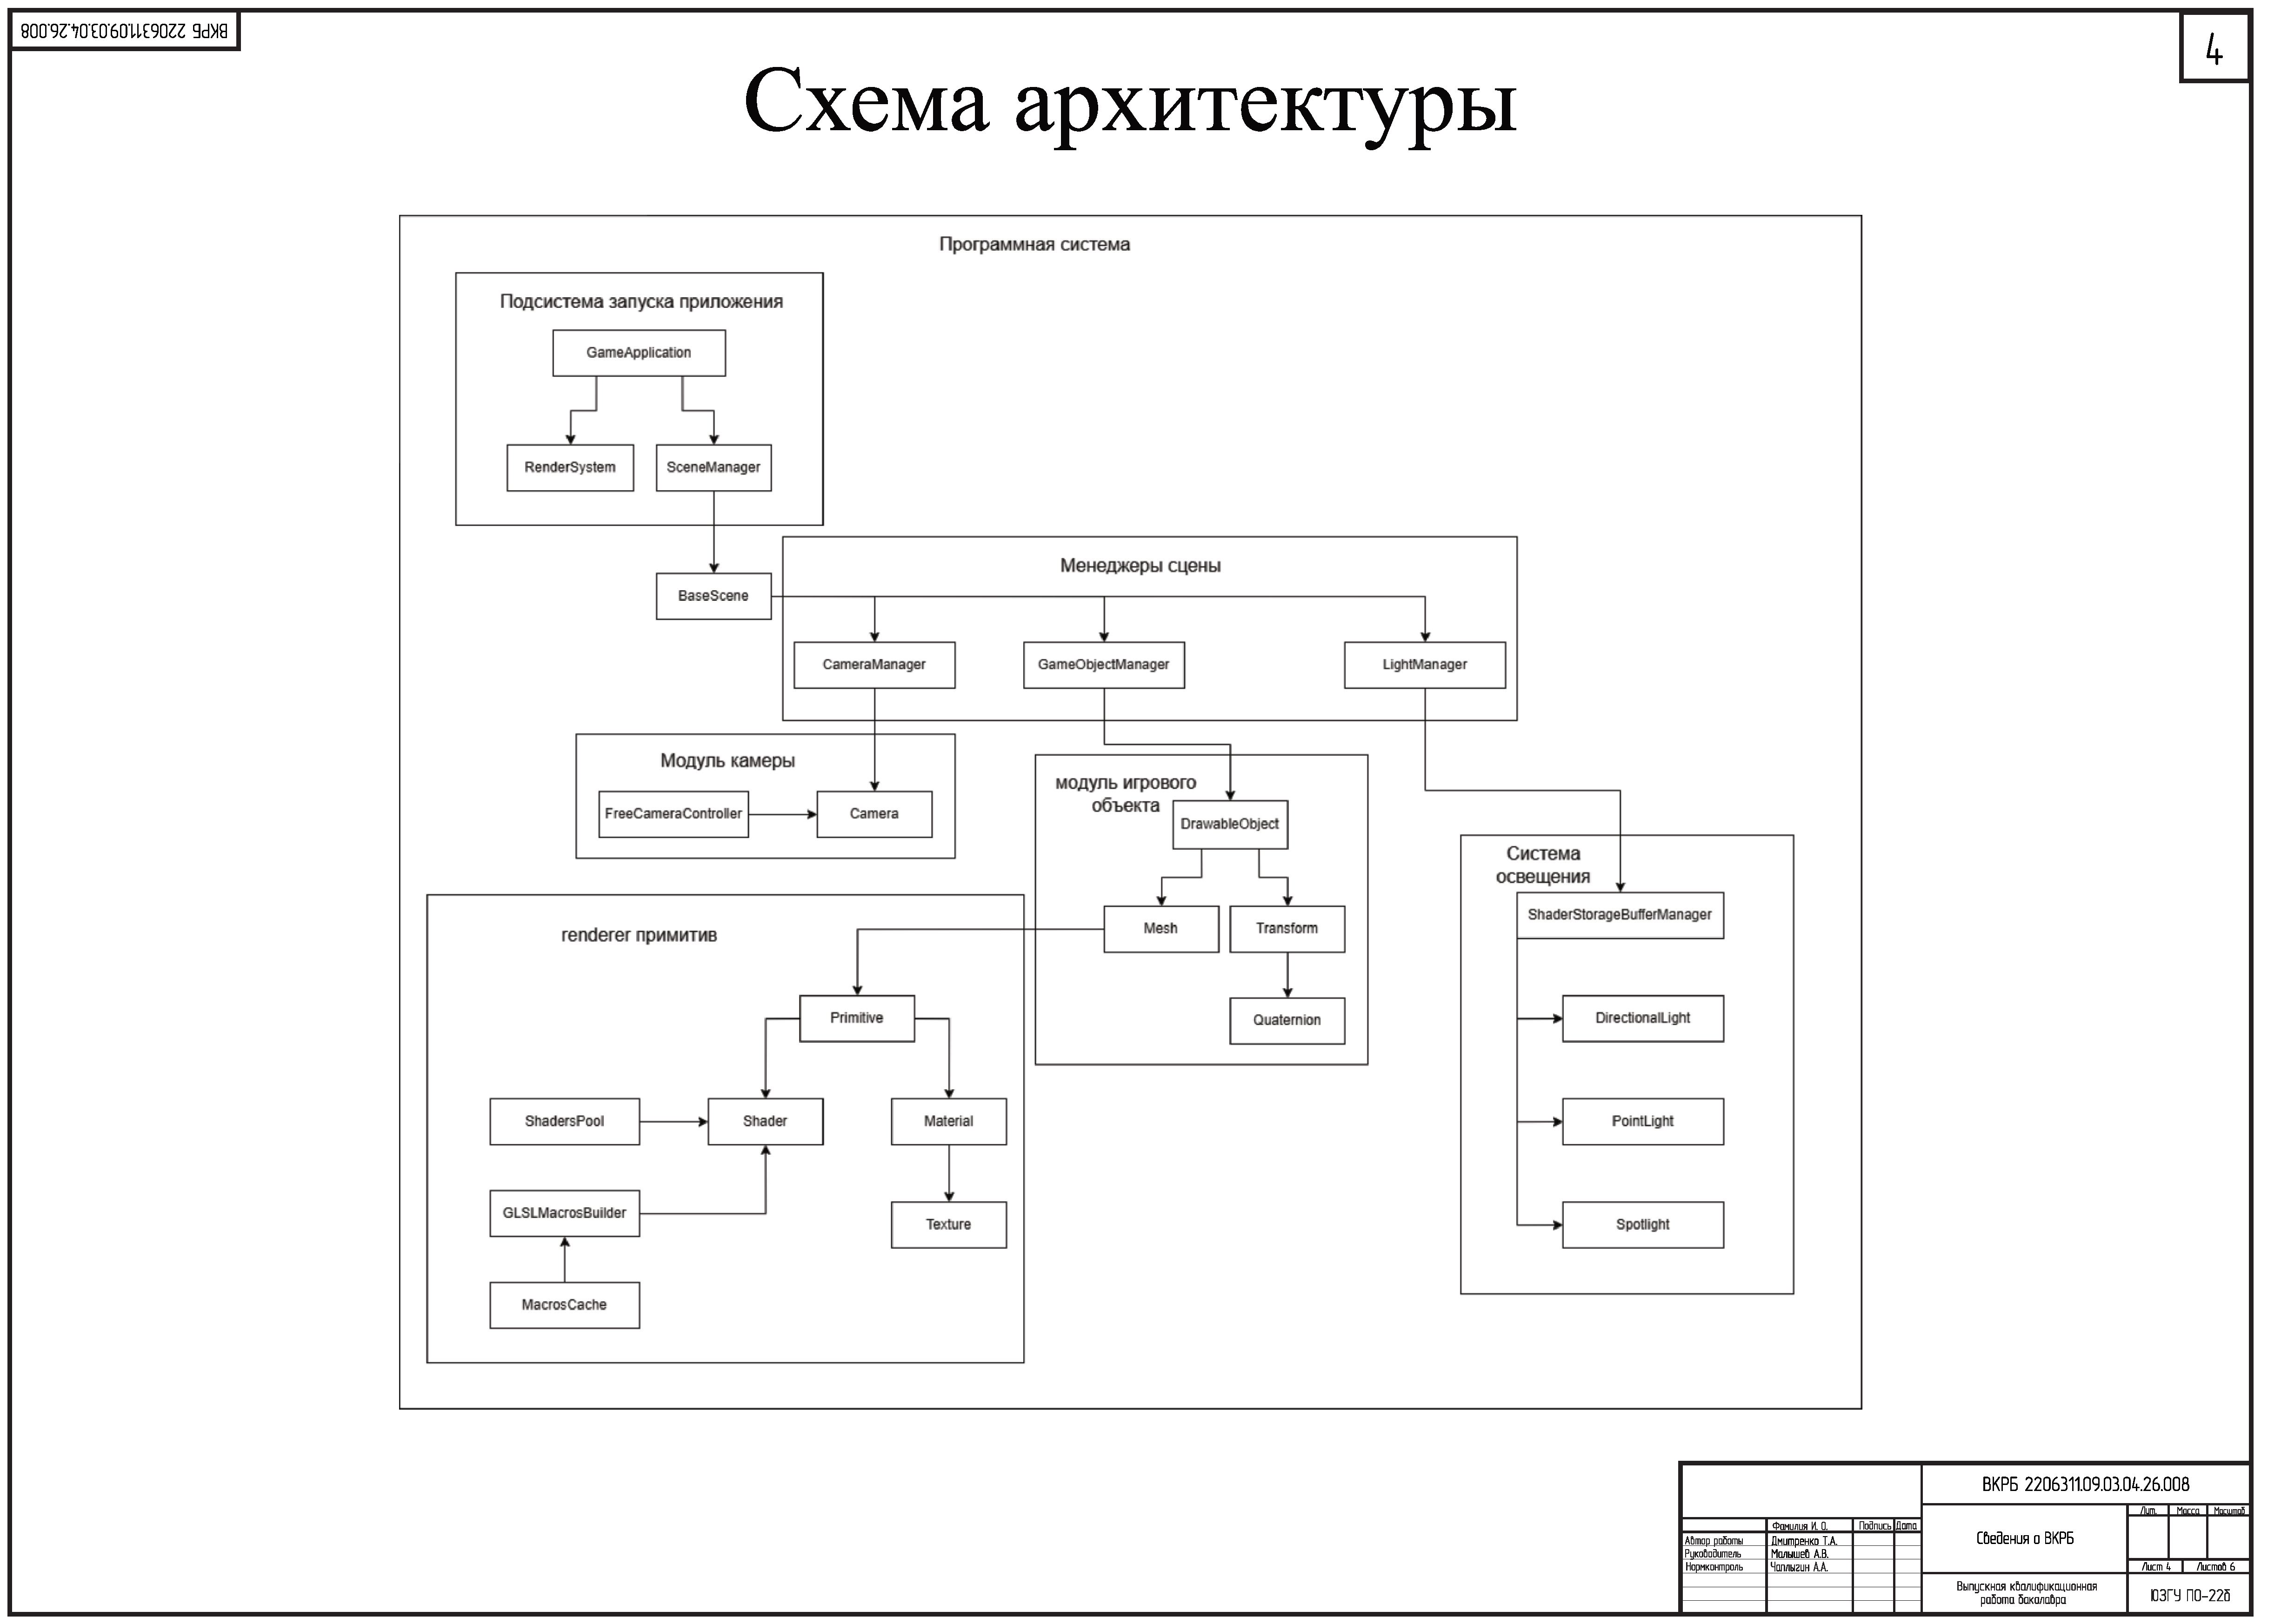
\includegraphics[width=0.82\linewidth]{images/4.eps}
    \заголовок{Еще плакат}
    \label{pl4:image}      
\end{плакат}

\begin{плакат}
	
\includegraphics[width=0.82\linewidth]{images/5.eps}
	\заголовок{Еще плакат}
	\label{pl5:image}      
\end{плакат}

\begin{плакат}
	
\includegraphics[width=0.82\linewidth]{6.eps}
	\заголовок{Еще плакат}
	\label{pl6:image}      
\end{плакат}

\end{landscape}
}\fi
\ifПрактика{}\else{\input{Код}}\fi
\end{document}
